\chapter{Non-contact estimation of vital signs}
\section{Introduction} 

The introduction of digital cameras into clinical image monitoring and diagnosis systems has allowed for tracking of changes in the vital signs of patients without contact with the individual. Though a great development, most existing studies in video-based non-contact vital sign monitoring have been carried out in tightly controlled conditions, over short periods of time (typically up to a couple of minutes). Furthermore, most current algorithms require a person to be still to ensure reliable measurements. The robustness of methods for estimating vital signs is therefore challenged when processing video data recorded from patients under real-life conditions.

\section{Dataset}

The clinical study used to obtain data was part of a research programme in the Oxford University Hospitals NHS (National Health Service) Foundation Trust and the Oxford Biomedical Research Centre (BRC). For this study, pre-term infants (born at less than 37 weeks of gestation) were nursed in a designated study incubator in the high-dependency area of the Neonatal Intensive Care Unit (\gls{nicu}) at the John Radcliffe Hospital in Oxford. The clinical team recruited the infants based on the British Association of Perinatal Medicine's Categories of Care 2011. 

30 pre-term infants were monitored for up to four consecutive days without affecting regular patient care. The participants were double-monitored with a digital video camera and the standard patient monitoring devices. The study was performed during daytime under regular ambient light conditions. Full details of this study protocol are presented Villaroel \textit{et al} \cite{villarroel2019non}.

\subsection{Participant selection and Assessment}

Participants needed to satisfy all of the following criteria: born at less than 37 weeks of gestation; requiring high-dependency care; requiring continuous monitoring of heart rate, respiratory rate and oxygen saturation; and requiring to be nursed naked inside an incubator. The study excluded any infants who presented life-threatening conditions that prevented the continuous monitoring in the high-dependency area of the \gls{nicu}. Consent was required to be given by the babies’ parents prior to any recording. Parents whose infants fulfilled the inclusion criteria were approached by the study personnel (\gls{nicu} clinicians) and given full verbal and written information about the study.

\subsection{Study set-up}

The set up of all the research equipment (video recording and data storage) was designed to minimise the inconvenience to clinical staff during the study. The designated Giraffe OmniBed Carestation incubator (General Electric, Connecticut, USA) was modified by drilling a small hole in the top panel of the canopy to allow a video camera to be positioned inside the incubator's chamber in order to film the infants without reflection and attenuation from the perspex layer (see figure~\ref{babycam}).  The study allowed for video recording to be temporarily paused, or the video camera temporarily covered, at the discretion of clinical staff during some clinical procedures such as phototherapy (for treating jaundice—yellow appearance of the skin), intravenous (IV) cannulation or when the infants were taken out of the incubator for cuddling by their parents (kangaroo care). If the infants were to be transferred to another unit, video recording was terminated and data were recorded until that point.
All the standard patient monitoring and care were continued throughout the study session.

\begin{figure}[!ht]
    \centering
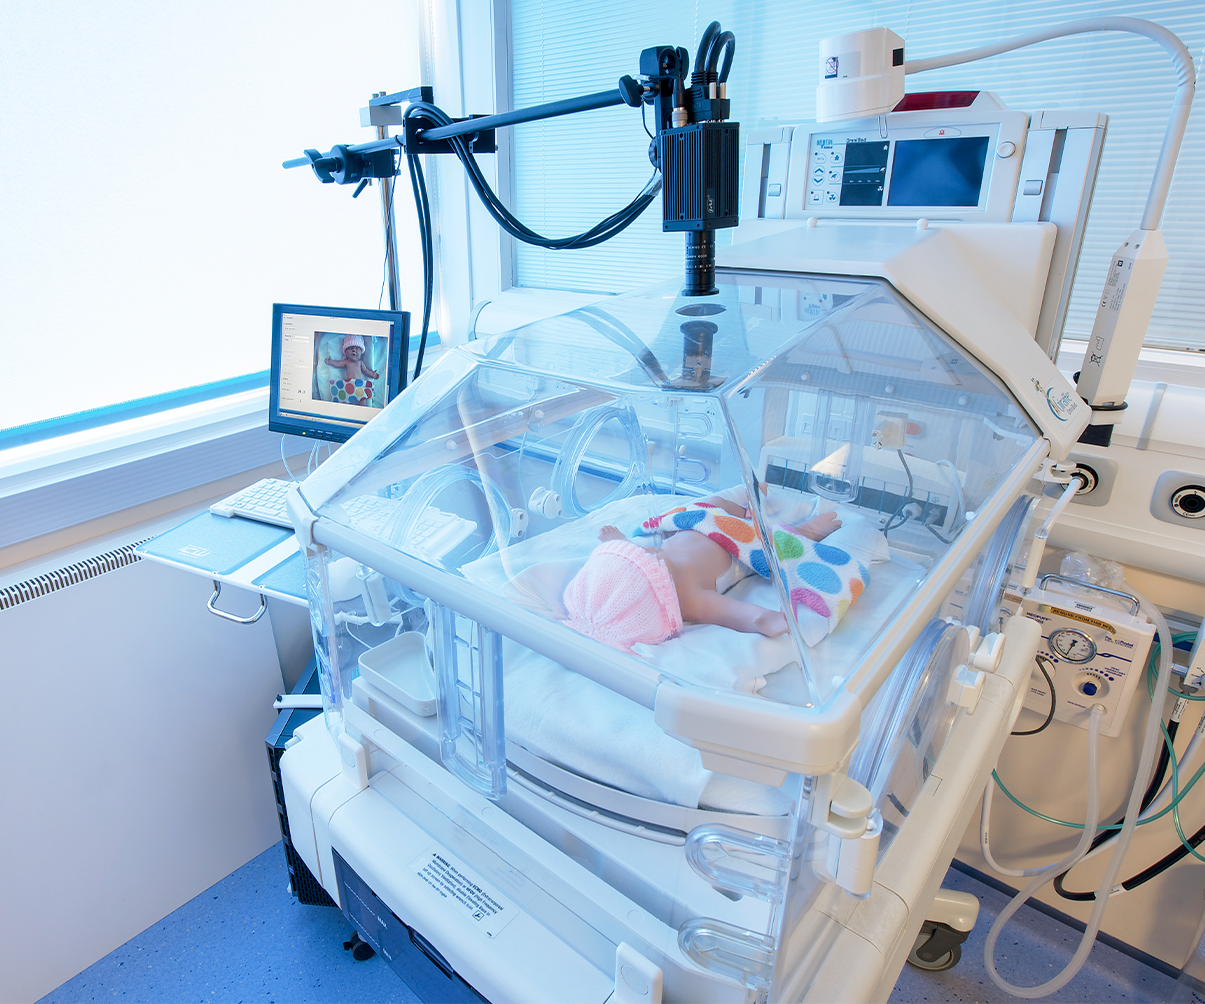
\includegraphics[width=0.45\linewidth,keepaspectratio=true]{nicu_babycam.png}
    \caption{A video camera positioned over a specifically-drilled hole in the top surface of the study incubator.}
    \label{babycam}
\end{figure}

\subsection{Instrumentation}

Video footage was recorded using a digital video camera positioned over the incubator inside which study infants were nursed (see figure~\ref{babycam}). This device was set to acquire 24-bit true colour images (Red/Green/Blue, 8-bit per colour) at a pre-set rate of 20 frames per second and at a resolution of 1628 × 1236 pixels. Conventional vital sign data was collected concurrently by the patient monitor as part of routine care. All conventionally-monitored signals were saved on a Philips patient monitor (Philips, Amsterdam, Netherlands)  and relayed to a separate workstation.

\subsection{Data Selection}

A single recording of a premature infant was selected to develop the algorithms. A 30-minute segment was selected from over 5 hours of overall recorded data for analysis. 40 minutes of Philips reference data (5 minutes before and 5 minutes after the video timestamps) was loaded around the requested camera time range to allow adjustment for differences in the Philips and camera timestamps.

\section{Heart rate estimation}

 
\subsection{Overview of the process}

\begin{figure}[!ht]
\centering
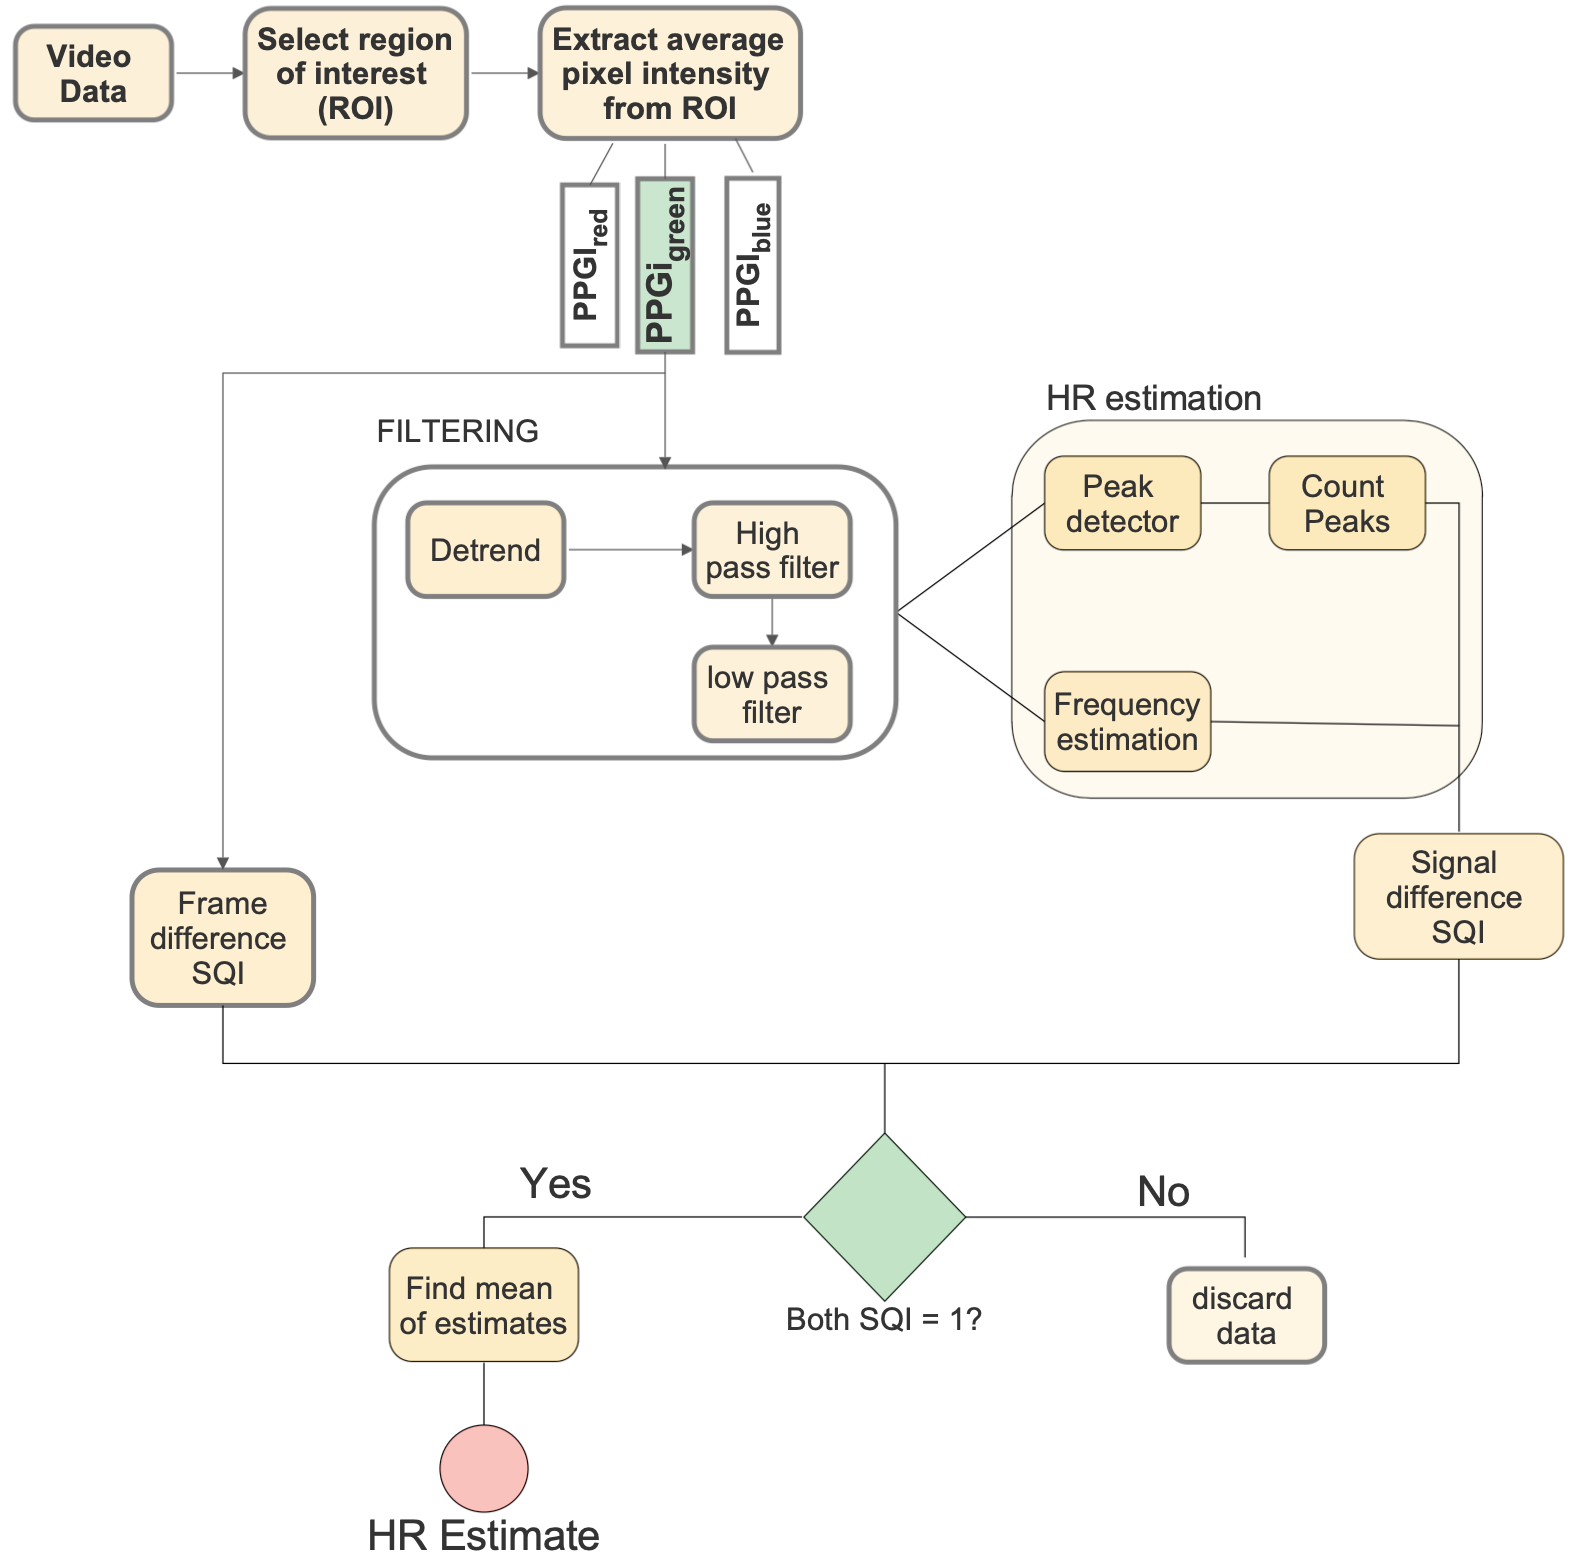
\includegraphics[width=0.7\linewidth,keepaspectratio=true]{nicu_Output_HR.png}
    \caption[Flow diagram outlining the process of estimating HR from a video data.]{Flow diagram outlining the process of estimating HR from video data.}
    \label{HRflow}
    \end{figure}
 
The extraction of the PPGi signal from the video camera data involved computing the average pixel intensity from within a region of interest (ROI), filtering the resulting signal to remove non-physiological frequencies and finally detecting peaks in the resulting waveform. 
 Motion artefacts resulting from the moving baby and moving camera were then discarded from the data using SQIs. 
 
\subsection{ROI Selection}
\label{roi exp}

One ROI was manually selected as shown in the red square in figure~\ref{ROI} by determining a 150 x 150 region on the back where skin was exposed. The mean pixel intensity within this \gls{roi} was computed for 30 minutes. Cardiac signals were extracted from the video based on the small color change on the skin that is consistent with the cardiac blood pulse. Cardiac signals were derived from the green channel as shown in figure~\ref{ppghr} because the green channel typically contains the strongest plethysmographic signal \cite{verkruysse2008remote}. 

\begin{figure}[!ht]
\centering
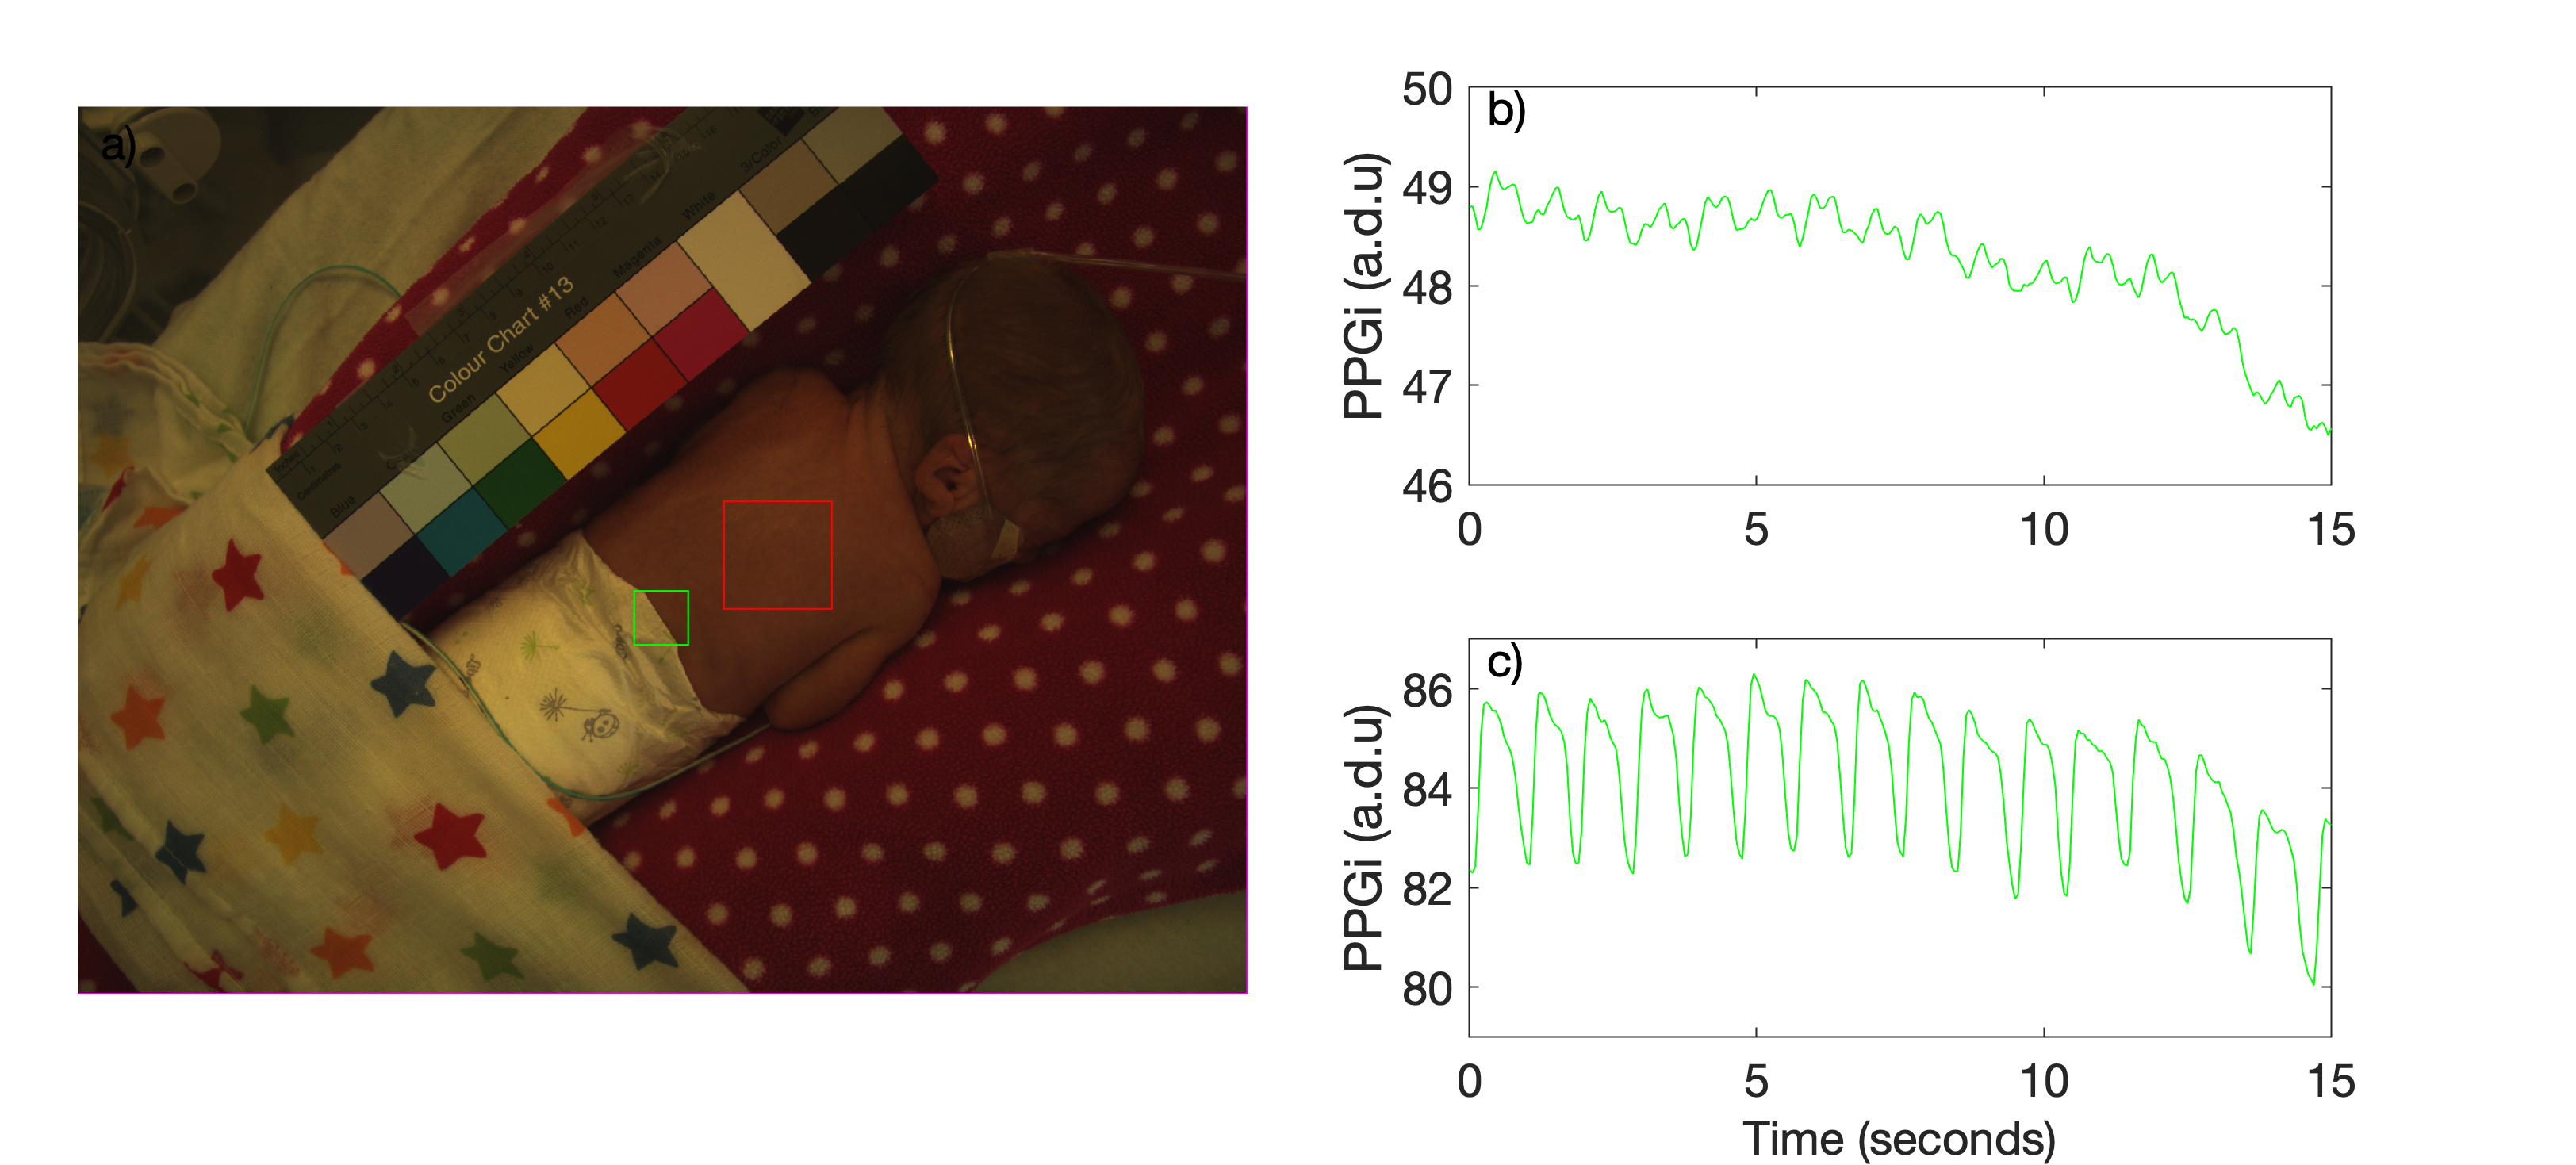
\includegraphics[width=0.6\linewidth,keepaspectratio=true]{nicu_ROI.png}
    \caption[Regions of Interest and PPGi signals.] {Regions of Interest and PPGi signals: a) Example video frame with ROIs for HR (in red) and RR (in green); b) Green PPGi signal extracted from the HR ROI; c) Green PPGi signal extracted from the RR ROI.} \label{ROI}
    \end{figure}

\subsection{Filtering}
\label{filter exp}

The PPGi signal was first de-trended. Subsequently 70$^{th}$ order zero-phase FIR filters with cut-off frequencies of 1.83 Hz (110 beats/min) and 2.92 Hz (175 beats/min) were designed and applied to the de-trended signal. The magnitude response of the resulting filters is shown in figure~\ref{HR_mag}. The result of applying the filters is shown in figure~\ref{HR_mag}.

\begin{figure}[!ht]
\centering
\includegraphics[width=0.5\linewidth,keepaspectratio=true]nicu_HR_magresponse.png}
    \caption[Magnitude responses.] {Magnitude responses. a) high-pass filter and b) low-pass filter.}
    \label{HR_mag}
    \end{figure}
 
\begin{figure}[!ht]
\centering
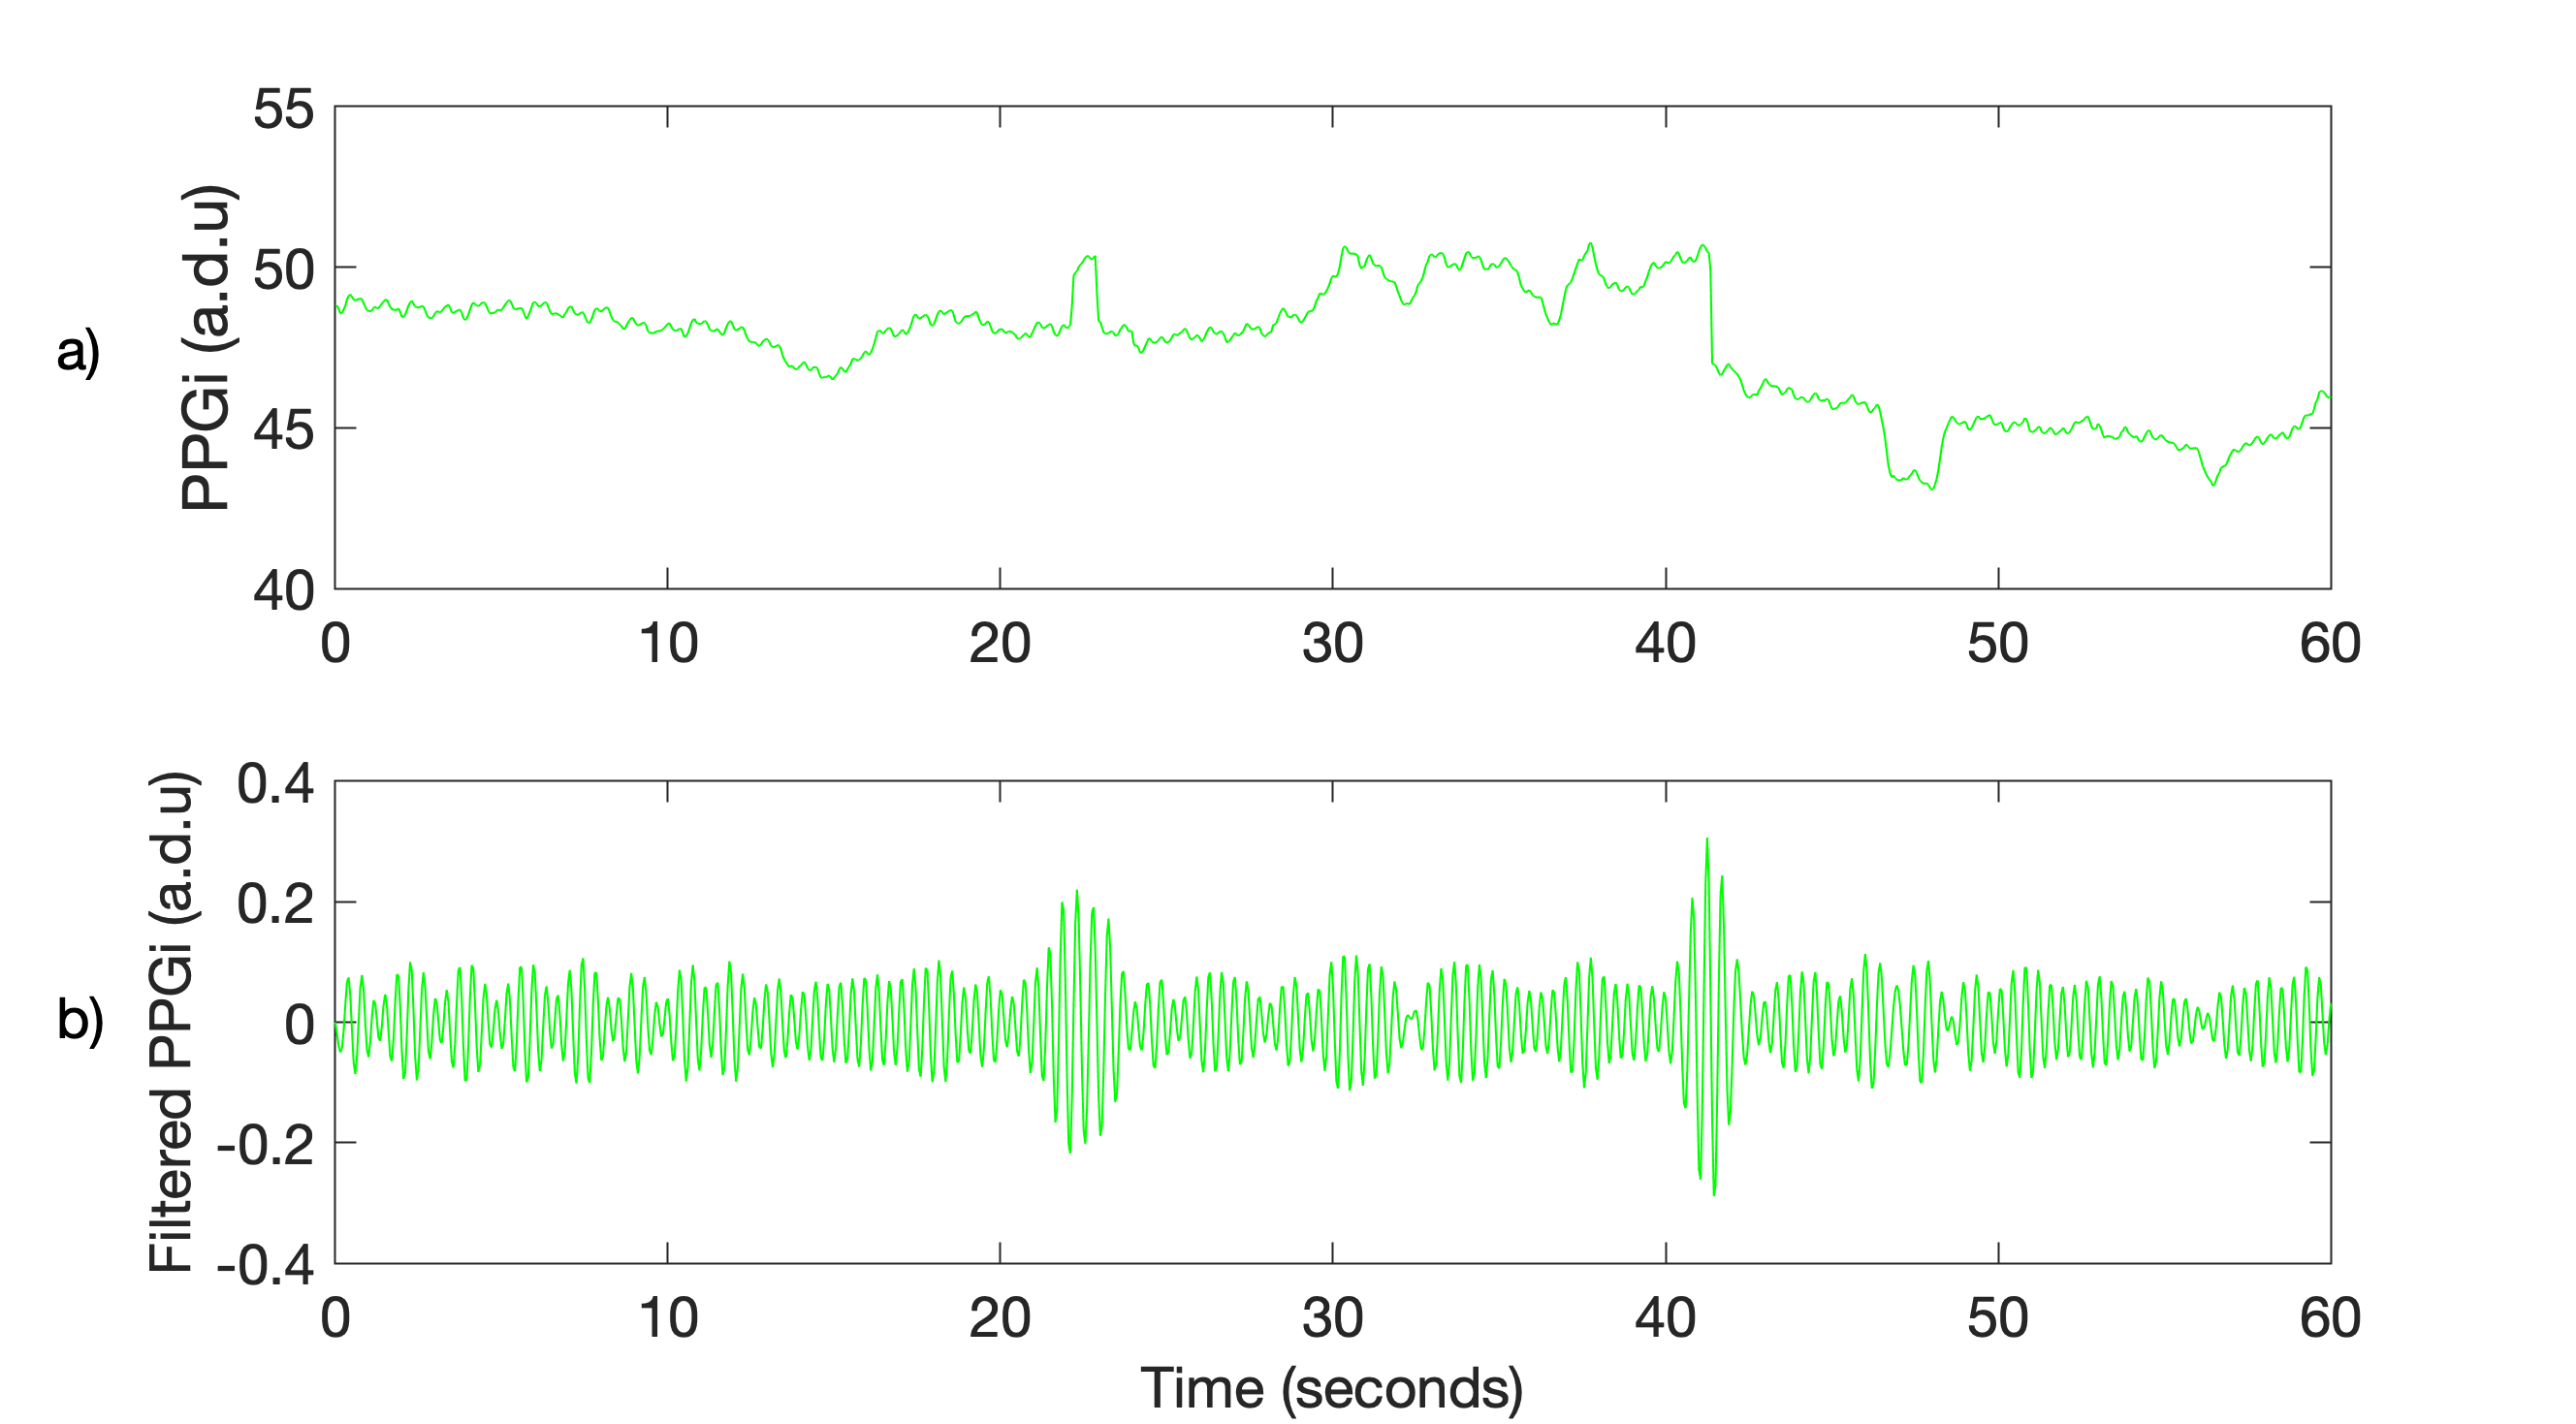
\includegraphics[[width=0.5\linewidth,keepaspectratio=true]{nicu_PPGi_hr.png}
    \caption[PPGi signal extracted from the HR ROI.] {PPGi signal extracted from the HR ROI. a) Green PPGi component; b) filtered green PPGi component.} \label{ppghr}
    \end{figure}
 
  \subsection{Peak-to-peak estimation}
 \label{peaks expl HR}
 
The filtered signal was re-sampled using a cubic spline at 75 Hz to provide better HR resolution as shown in figure~\ref{resahr}.
 
\begin{figure}[!ht]
\centering
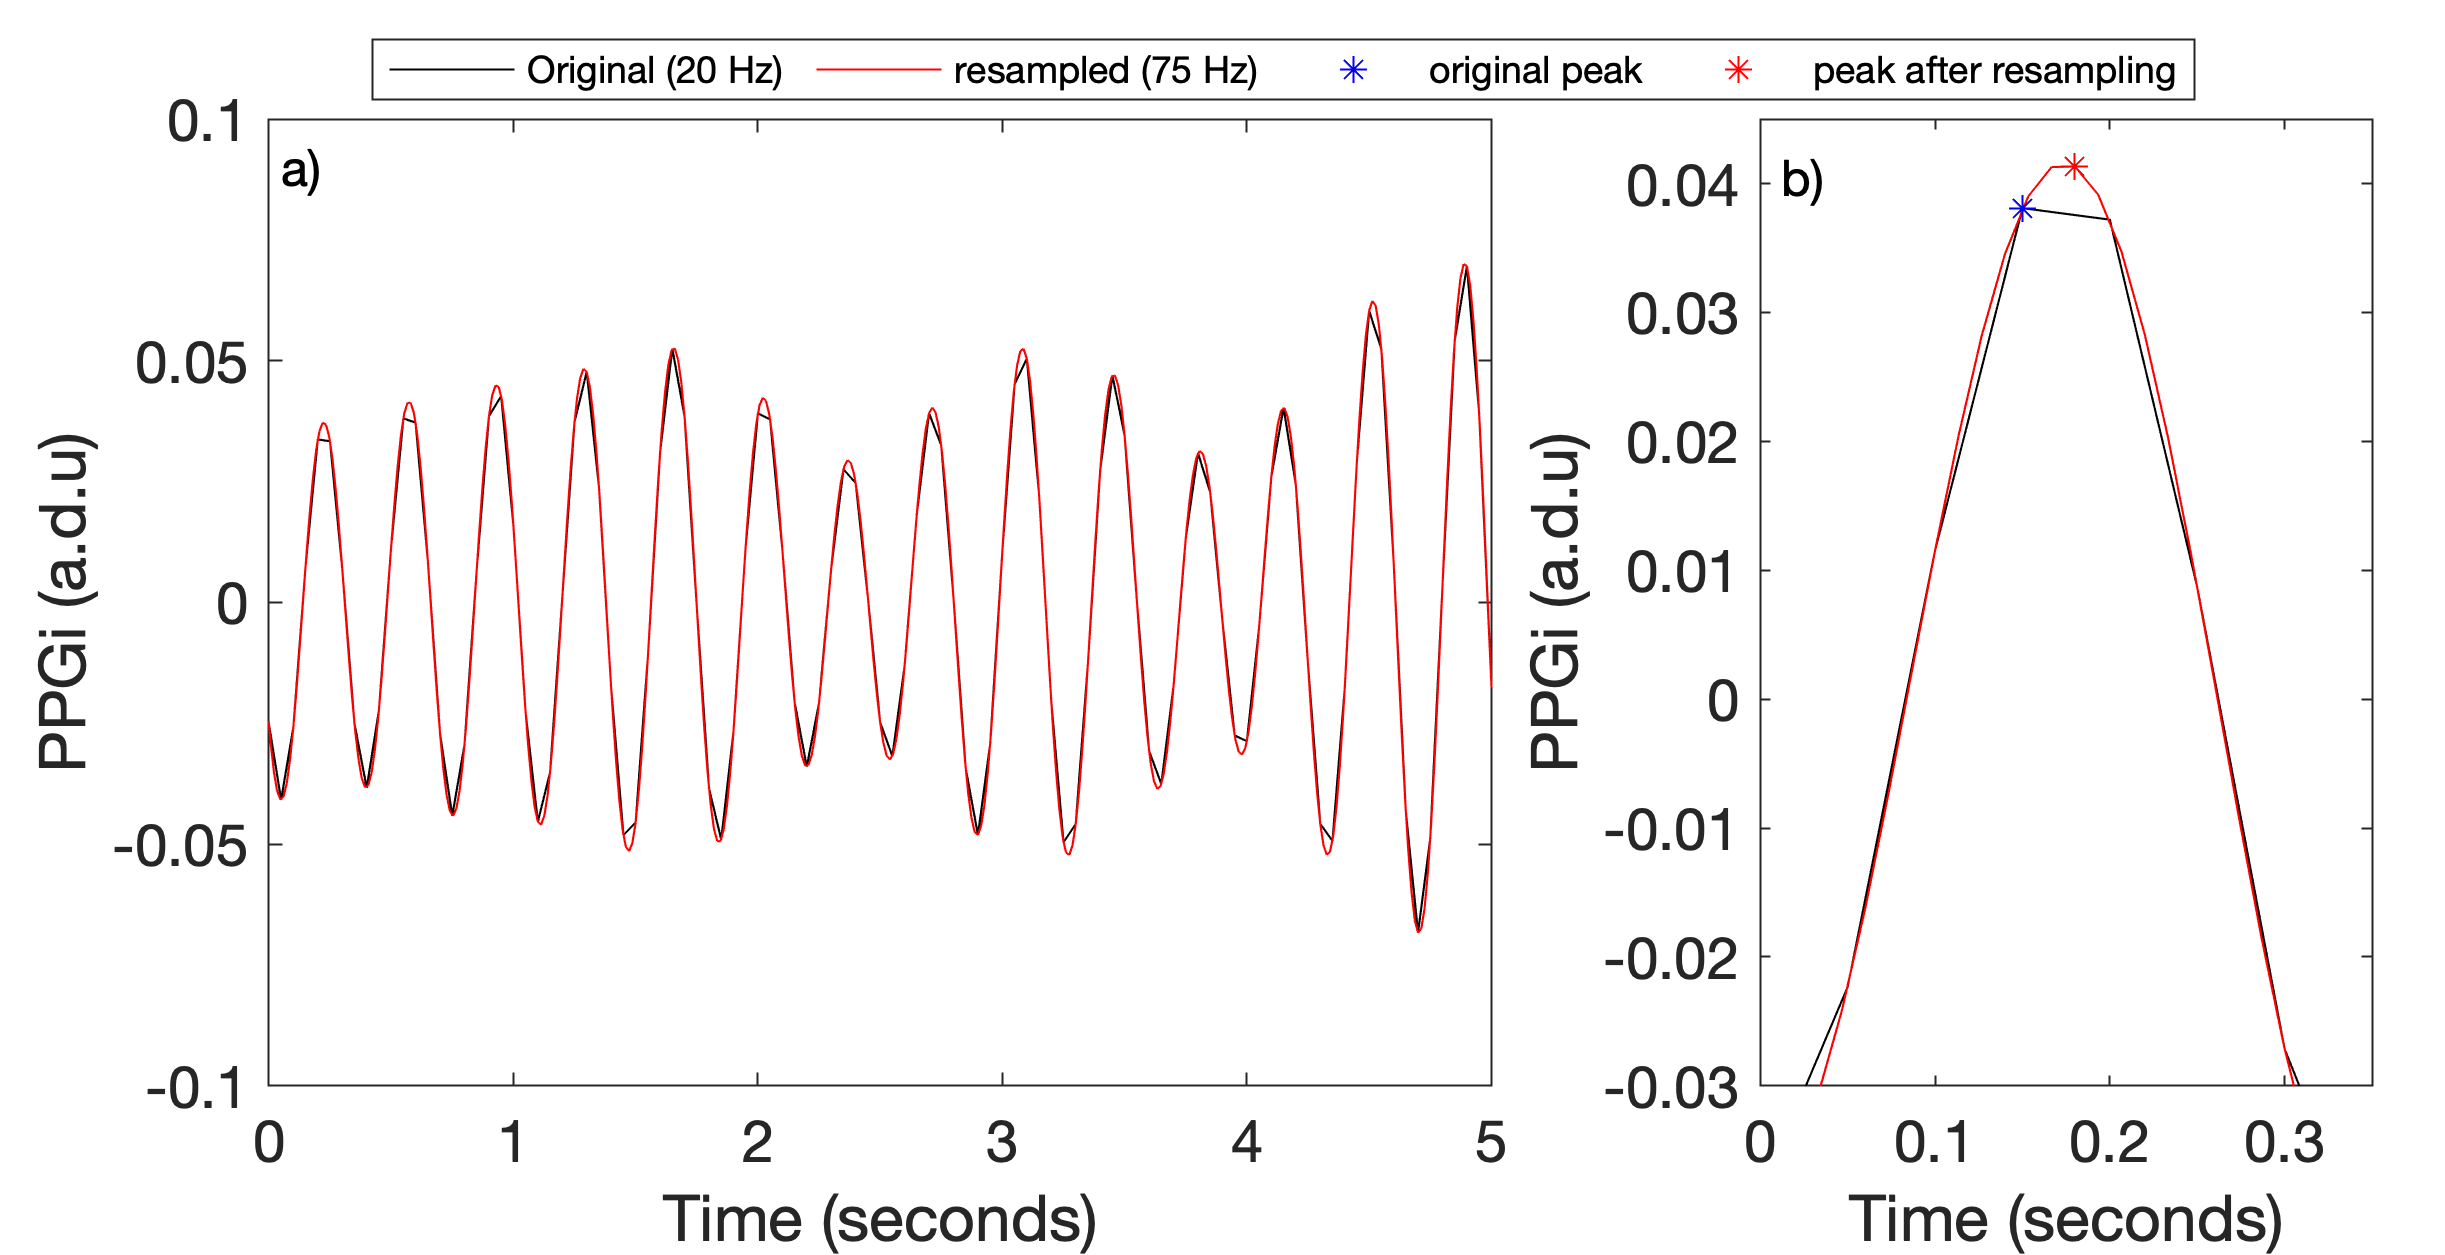
\includegraphics[width=0.5\linewidth,keepaspectratio=true]{nicu_resampled_hr.png}
      \caption[Reconstruction of a PPGi signal using cubic spline interpolation.] {Reconstruction of a PPGi signal using cubic spline interpolation. a) The original and re-sampled signals. b) Peaks detected using the original and re-sampled waveforms.} \label{resahr}
    \end{figure}

Peak-to-peak analysis was then performed on the re-sampled signal. This process involved identifying prominent maximum and minimum points in the signal to represent signal amplitude. The algorithm used for peak detection first identified a peak as the $i _{th}$ sample in a time series $ts$ if: 
\begin{equation}
	ts(i) > ts(i-1)\textrm{ \textbf{and} } ts(i) > ts(i+1)
\end{equation}
To avoid reporting erroneous peaks due to noise, identified peaks were kept where:

\begin{equation}
	ts(i_{peak})  > MinPeakHeight
\end{equation}

where MinPeakHeight was set to a signal intensity of -0.02, based on manually observing the minimum height of waveform peaks in low intensity segments of the recording. Remaining peaks were retained if:

\begin{equation}
	i_{peak_{n}} - i_{peak_{n-1}}  >  MinPeakDistance
\end{equation}

where MinPeakDistance was set to give a refractory period (a recovery time after each peak) of 23 samples at 75Hz (corresponding to 200 beats/minute) based on the reference vital-sign data for the session. Finally, peaks were selected where:

\begin{equation}
	prom(i_{peak}) > MinPeakProminence
\end{equation}

where $prom$ is the prominence of a peak, defined as the height of the peak relative to neighbouring troughs. Here, MinPeakProminence was set to a signal intensity of 0.005 based on manually observing peak prominences in several example recording segments. The algorithm then returned a vector containing the location and magnitude of each peak as shown in Fig.~\ref{HR_peaks}c. The FFT panels show a peak at 2.8Hz, corresponding to a HR of approximately 168 beats/minute. The reference HR recorded by the Philips monitor was 167.9 beats/minute.

\begin{figure}[!ht]
\centering
\includegraphics[width=0.6\linewidth,keepaspectratio=true]nicu_HR_peaks.png}
    \caption[30-second analysis of filtered cardiac signals from the video camera data.]{30-second analysis of filtered cardiac signals from the video camera data: a) Input signal; b) signal after filtering and c) peak detection. The FFT panels show a peak at 2.8Hz, corresponding to a HR of approximately 168 beats/minute. The reference HR recorded by the Philips monitor was 167.9 beats/minute.}
    \label{HR_peaks}
    \end{figure}
 
 \subsection{Initial HR estimates}
 
 Two methods were used to compute HR from the video camera data. Peak-to-peak intervals, caused by...allowed the estimation of HR. The second method, Frequency estimation, used the frequency of the most prominent FFT peak to estimate HR.

\subsubsection{Beat Counting}

For this method, the time value of each peak was subtracted from the time value of the succeeding peak to get raw peak-to-peak time intervals. These were then converted into heart rates by using equation~\ref{HRequation}. Rolling means were computed for every 20-second window, sliding by 1 second. This process was also applied to the Phillips reference signal to ensure our estimates were comparable.
\begin{equation}
    \label{HRequation}
HR = \frac{60}{peak\_to\_peak\_interval}
\end{equation}

\subsubsection{Frequency estimation}

Each 20-second window, sliding by 1 second, was de-trended and the Fast Fourier Transform (FFT) was computed. Figure~\ref{HR_peaks} shows the cardiac signal and its associated frequency spectra. Each spectrum plots the magnitude of the FFT against frequency. The figure shows that the selected green channel contains a prominent low-frequency content and cardiac component (the latter at approximately 2.8 Hz, or 168 beats/minute). The low frequency is filtered out as shown in the FFT plot of figure~\ref{HR_peaks}b. The frequency of the remaining FFT peak was taken as an estimate for the HR frequency in that window.

\subsection{Signal Quality assessment}
\label{sqis expl}

Two signal quality index algorithms are proposed: signal difference and frame difference. 
Figure~\ref{SQI_vidHR} shows a 120-second sample plot of the two proposed methods.

\subsubsection{Signal Difference SQI}

The agreement between the two estimation methods (peak-to-peak and FFT) was used to create an HR difference SQI. This SQI was set to 1 if the two estimates were within 3 beats/min, and set to 0 otherwise.

\subsubsection{Frame Difference SQI}

A frame difference signal was created by comparing the intensity of the pixels between two subsequent frames. This was done by taking the mean of the absolute differences between each pair of pixels. 

\begin{equation}
	diff_{frame} =\dfrac{\sum_{x}^{}\sum_{y}^{}\textrm{abs}(frame(x,y,i) - frame(x,y,i - 1))}{\textrm{len}(x) \times \textrm{len}(y)} 
\end{equation}

where $frame(x,y,i)$ is a pixel with coordinates x and y in the i$^{th}$ frame, len($x$) is the width of the frame and len($y$) is the height of the frame. Changes in lighting or movement should cause bigger changes in intensity, indicating regions of poor signal quality. If this difference in pixel intensity was greater than a threshold value  of mean + 1.6 \times standard deviation, the SQI was set to 0.

\begin{figure}[!ht]
    \centering
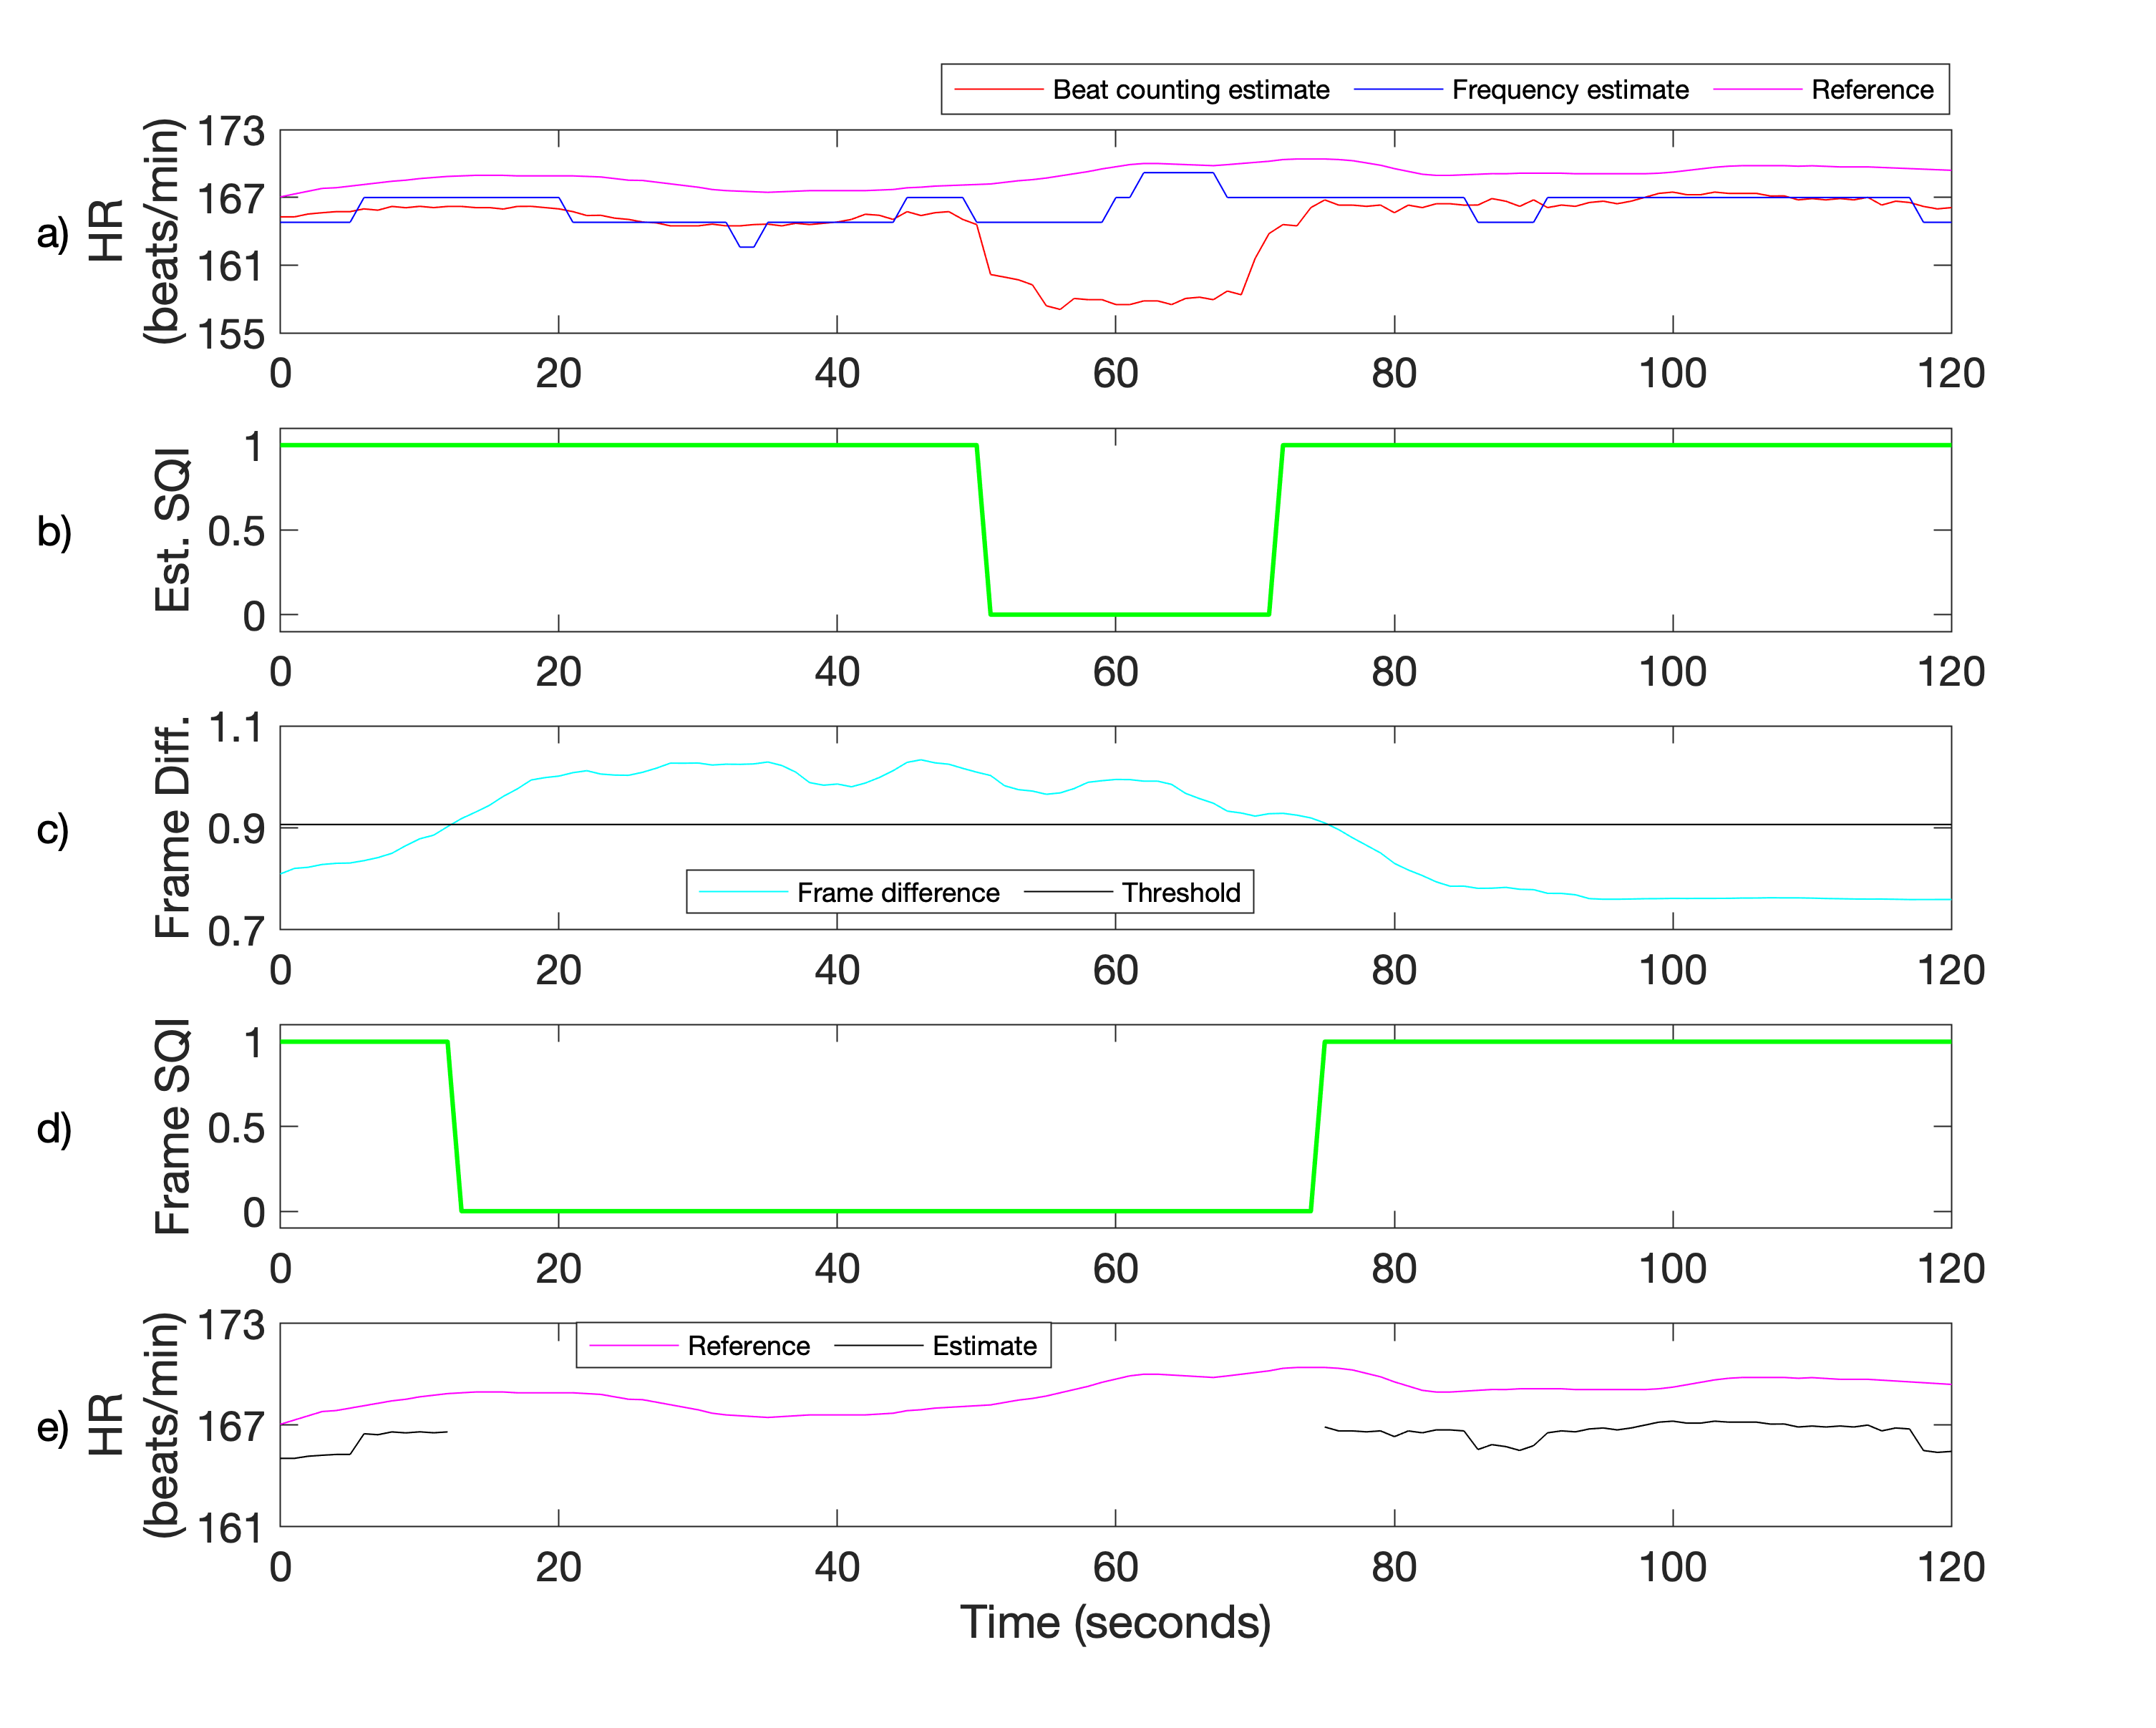
\includegraphics[width=0.6\linewidth,keepaspectratio=true]{nicu_SQI_vidHR.png}
    \caption[Using SQI to discard noisy data. Periods of high movement were removed using two signal quality indices.]{Using SQI to discard noisy data. Periods of high movement were removed using signal quality indices. a) Beat counting and frequency estimates in comparison to the reference HR estimate; b) Signal difference SQI; c) Frame difference; d) Frame difference SQI; e) Comparison between reference and HR estimate.}
    \label{SQI_vidHR}
\end{figure}

 \subsection{Estimating HR}
 
Following the signal quality assessment, HR was estimated using a 20-second sliding window with a step size of 1 second. If either the signal or frame difference SQIs were 0, the window was taken as a poor-quality window and was discarded. If both SQIs were equal to 1, HR for that window was estimated as:

\begin{equation}
HR_{estimate} = \frac{HR_{FFT} + HR_{peak-to-peak} }{2}	
\end{equation} 
    
\section{Respiratory rate estimation}
\subsection{Overview of the process}
    \label{sec:camera_rr_est_overview} 

\begin{figure}[!ht]
    \centering
\includegraphics[width=0.6\linewidth,keepaspectratio=true]nicu_Output_RR.png}
    \caption{Flow diagram outlining the process of estimating RR from video data.}
    \label{fig:camera_rr_est_overview}
\end{figure}

Figure~\ref{fig:camera_rr_est_overview} presents an overview of the methods used to estimate RR from video camera data. The raw PPGi signal was extracted by taking the mean of the pixel intensity from a ROI over the patient's back. Two digital filters were used to suppress frequency components below 0.25 Hz and above 1.42 Hz, corresponding to a respiratory rate range approximately between 15 to 85 breaths/min. A peak detection method was applied to filtered the signal to identify prominent points. Subsequently, the quality of the PPGi signal was analysed to identify areas of good-quality respiratory signal. RR estimates were computed for periods for which the PPGi signal was judged to be of good quality.

\subsection{ROI Selection}
\label{roirr}

Breathing causes volume changes of the infant's lungs which in turn causes movement of the body. This movement can be captured by a video camera from areas containing exposed skin or covered by tight-fitting clothing such as a nappy. Respiratory signals can therefore be extracted from the respiration induced chest/abdomen motion. One ROI of size 75 x 75 pixels, was manually selected and the mean pixel intensity within the selected ROI was computed for each video frame (see figure~\ref{ROI}). As with HR, only the green channel was used for processing.
 
\subsection{Filtering}
\label{filteringrr}

The respiratory signal extracted from the selected ROI was de-trended by fitting a straight line to the data using linear regression and subtracting this straight line from the data. The de-trended data was further processed by applying two IIR filters  to remove low and high frequency noise from the signal. A 2$^{nd}$ order high-pass and low-pass filter were designed with cut-off frequencies of 0.25 Hz (15 breaths/min) and 1.42 Hz (85 breaths/min), respectively (see figure~\ref{filterrr}). The result of applying the filters to a sample time series extracted from the video camera data is shown in figure~\ref{RR_peaks}.

\begin{figure}[!ht]
\centering
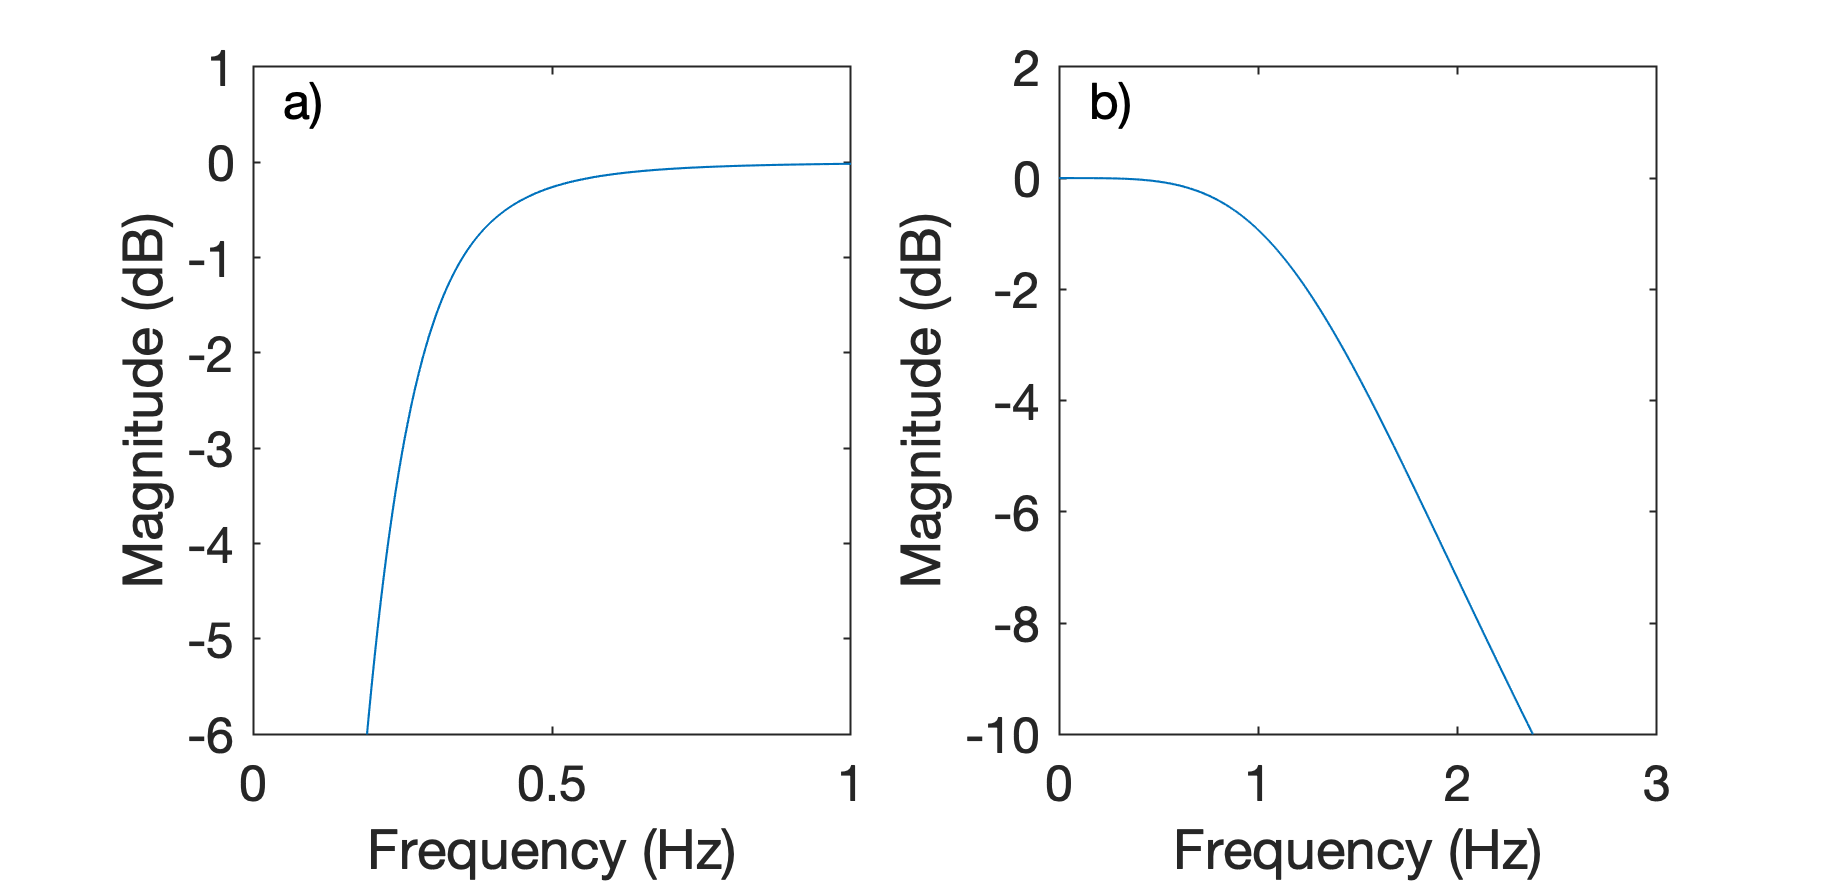
\includegraphics[width=0.6\linewidth,keepaspectratio=true]{nicu_RR_magresponse.png}
    \caption[Magnitude responses for extracting a respiratory signal from the video camera data.]{Magnitude responses for extracting a respiratory signal from the video camera data. a) High-pass filter and b) low-pass filter.}
\label{filterrr}
    \end{figure}

\subsection{Peak-to-peak estimation}
    \label{RR_peaks2peak}
    
The filtered signal was re-sampled using a cubic spline at 75 Hz to provide better RR resolution. Local peaks found were then found by using the the algorithms described in section~\ref{peaks expl HR}. This analysis was done using MinPeakDistance of 12.0 ms (83.3 breaths/min), MinPeakHeight of -15.0 and MinPeakProminence of 0.05. The algorithm then returned a vector containing the result of the location and magnitude of each peak as shown in figure Fig.~\ref{RR_peaks}.

\begin{figure}[!ht]
\centering
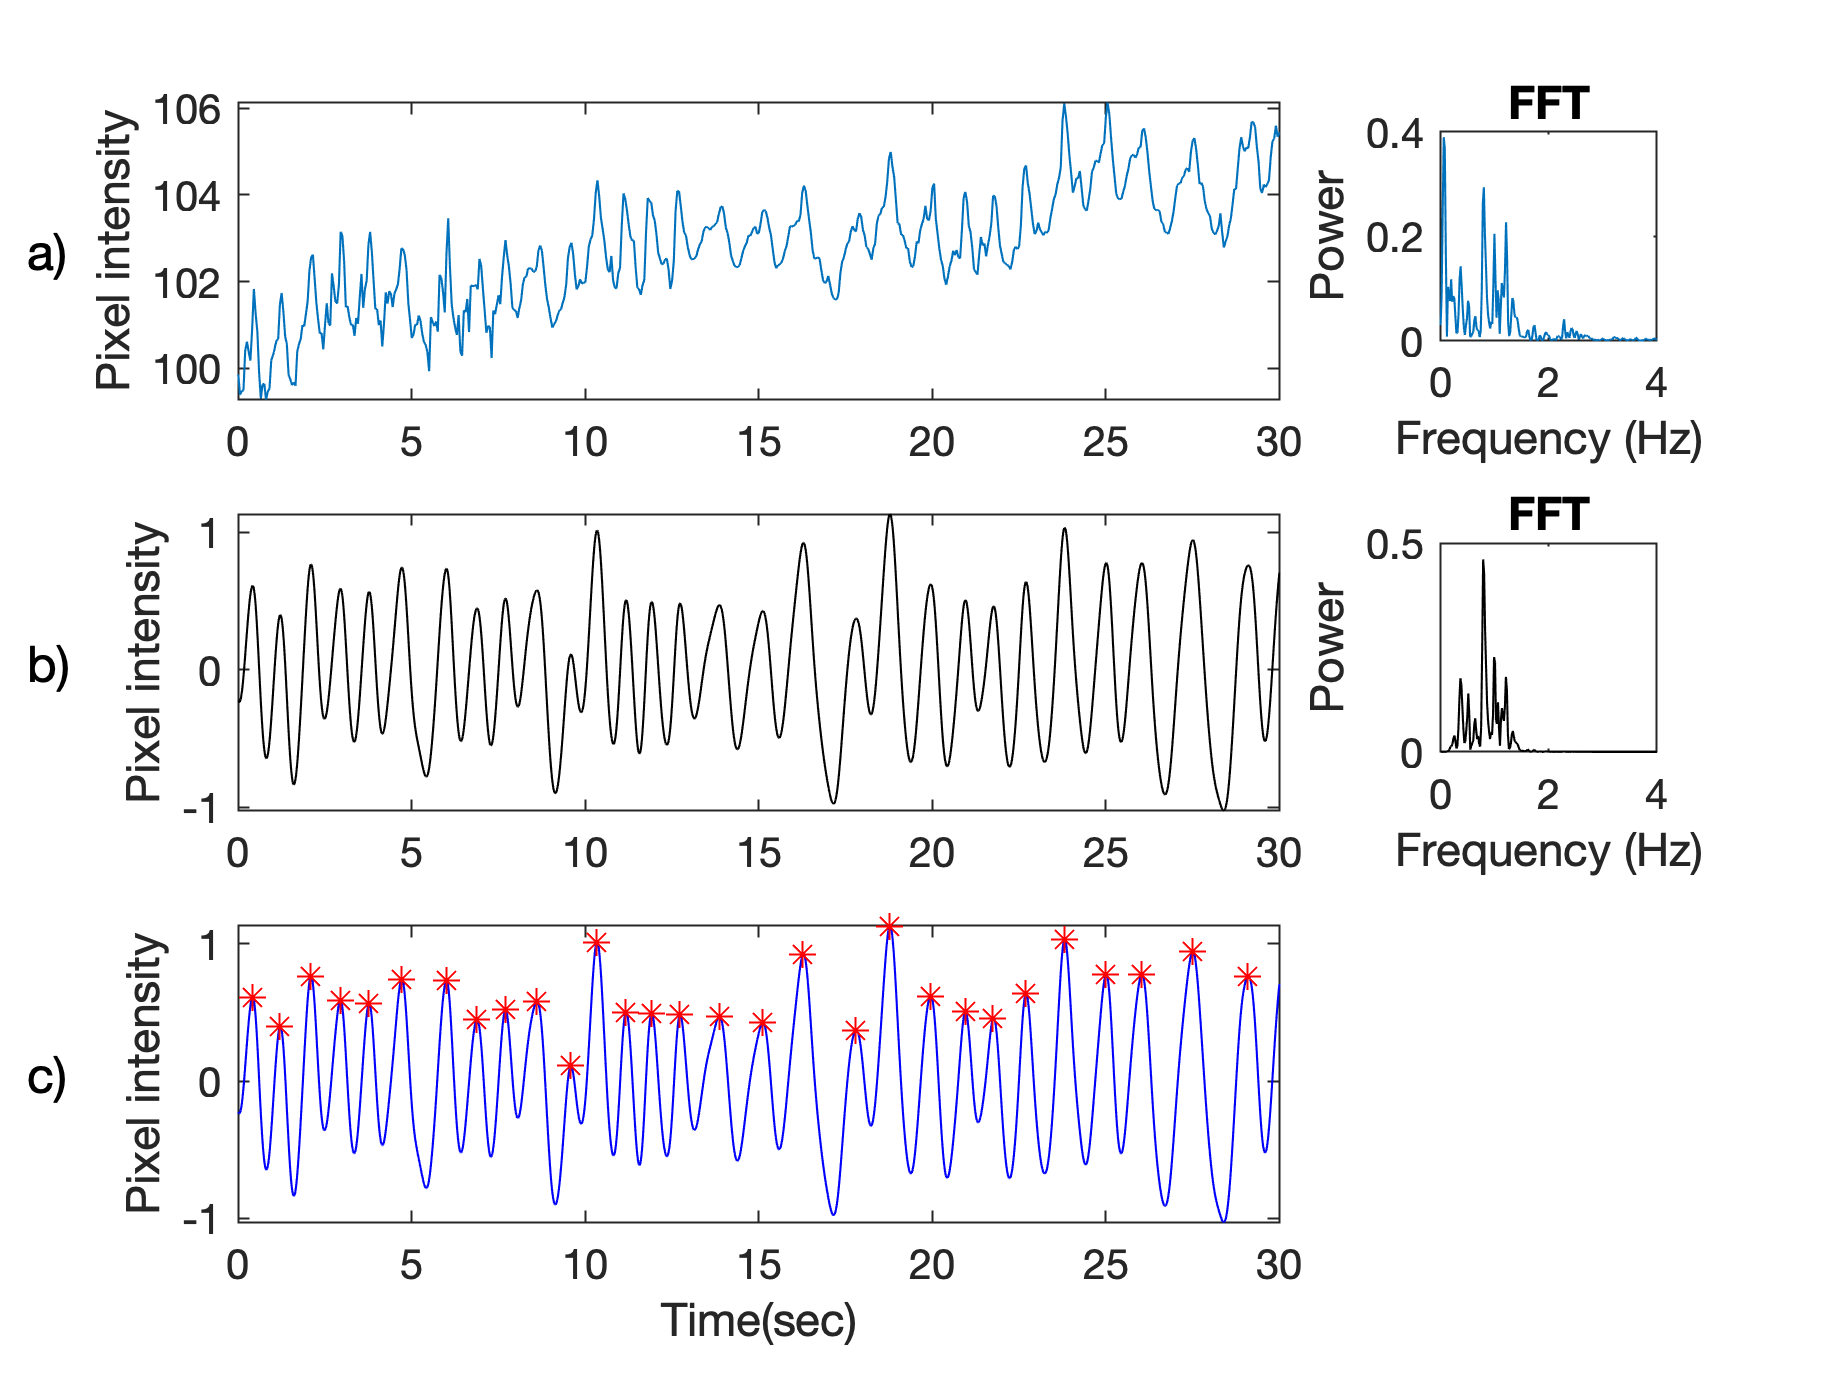
\includegraphics[width=0.6\linewidth,keepaspectratio=true]{nicu_RR_peaks.png}
    \caption[Peak detection for a 30-second sample respiratory signal.] {Peak detection for a 30-second sample respiratory signal. a) Input signal; b) Signal after filtering and c) detected peaks.}
    \label{RR_peaks}
    \end{figure}
 
 The time value of each peak was subtracted from the time value of the succeeding peak to get raw breath length estimates. These were then converted into respiratory rates by using equation~\ref{RRequation}. Rolling medians were computed over a 40-second window sliding by 5 second. This process was also applied to the Phillips reference signal to ensure our estimates were comparable.
 
 \begin{equation}
 RR = \frac{60}{breath\_length}
\label{RRequation}
\end{equation}

\subsection{Respiratory signal quality assessment}
\label{rrsqi}
\subsubsection{Frame Difference SQI}

 Changes in lighting or movement caused large changes in light intensity recorded by the video camera. The pixel intensity of every frame was averaged and subtracted to that of the succeeding frame. If the difference in pixel intensity was greater than a threshold value, the SQI was set to 0 as demonstrated in figure~\ref{SQI_vidRR}.
 
\begin{figure}[!ht]
    \centering
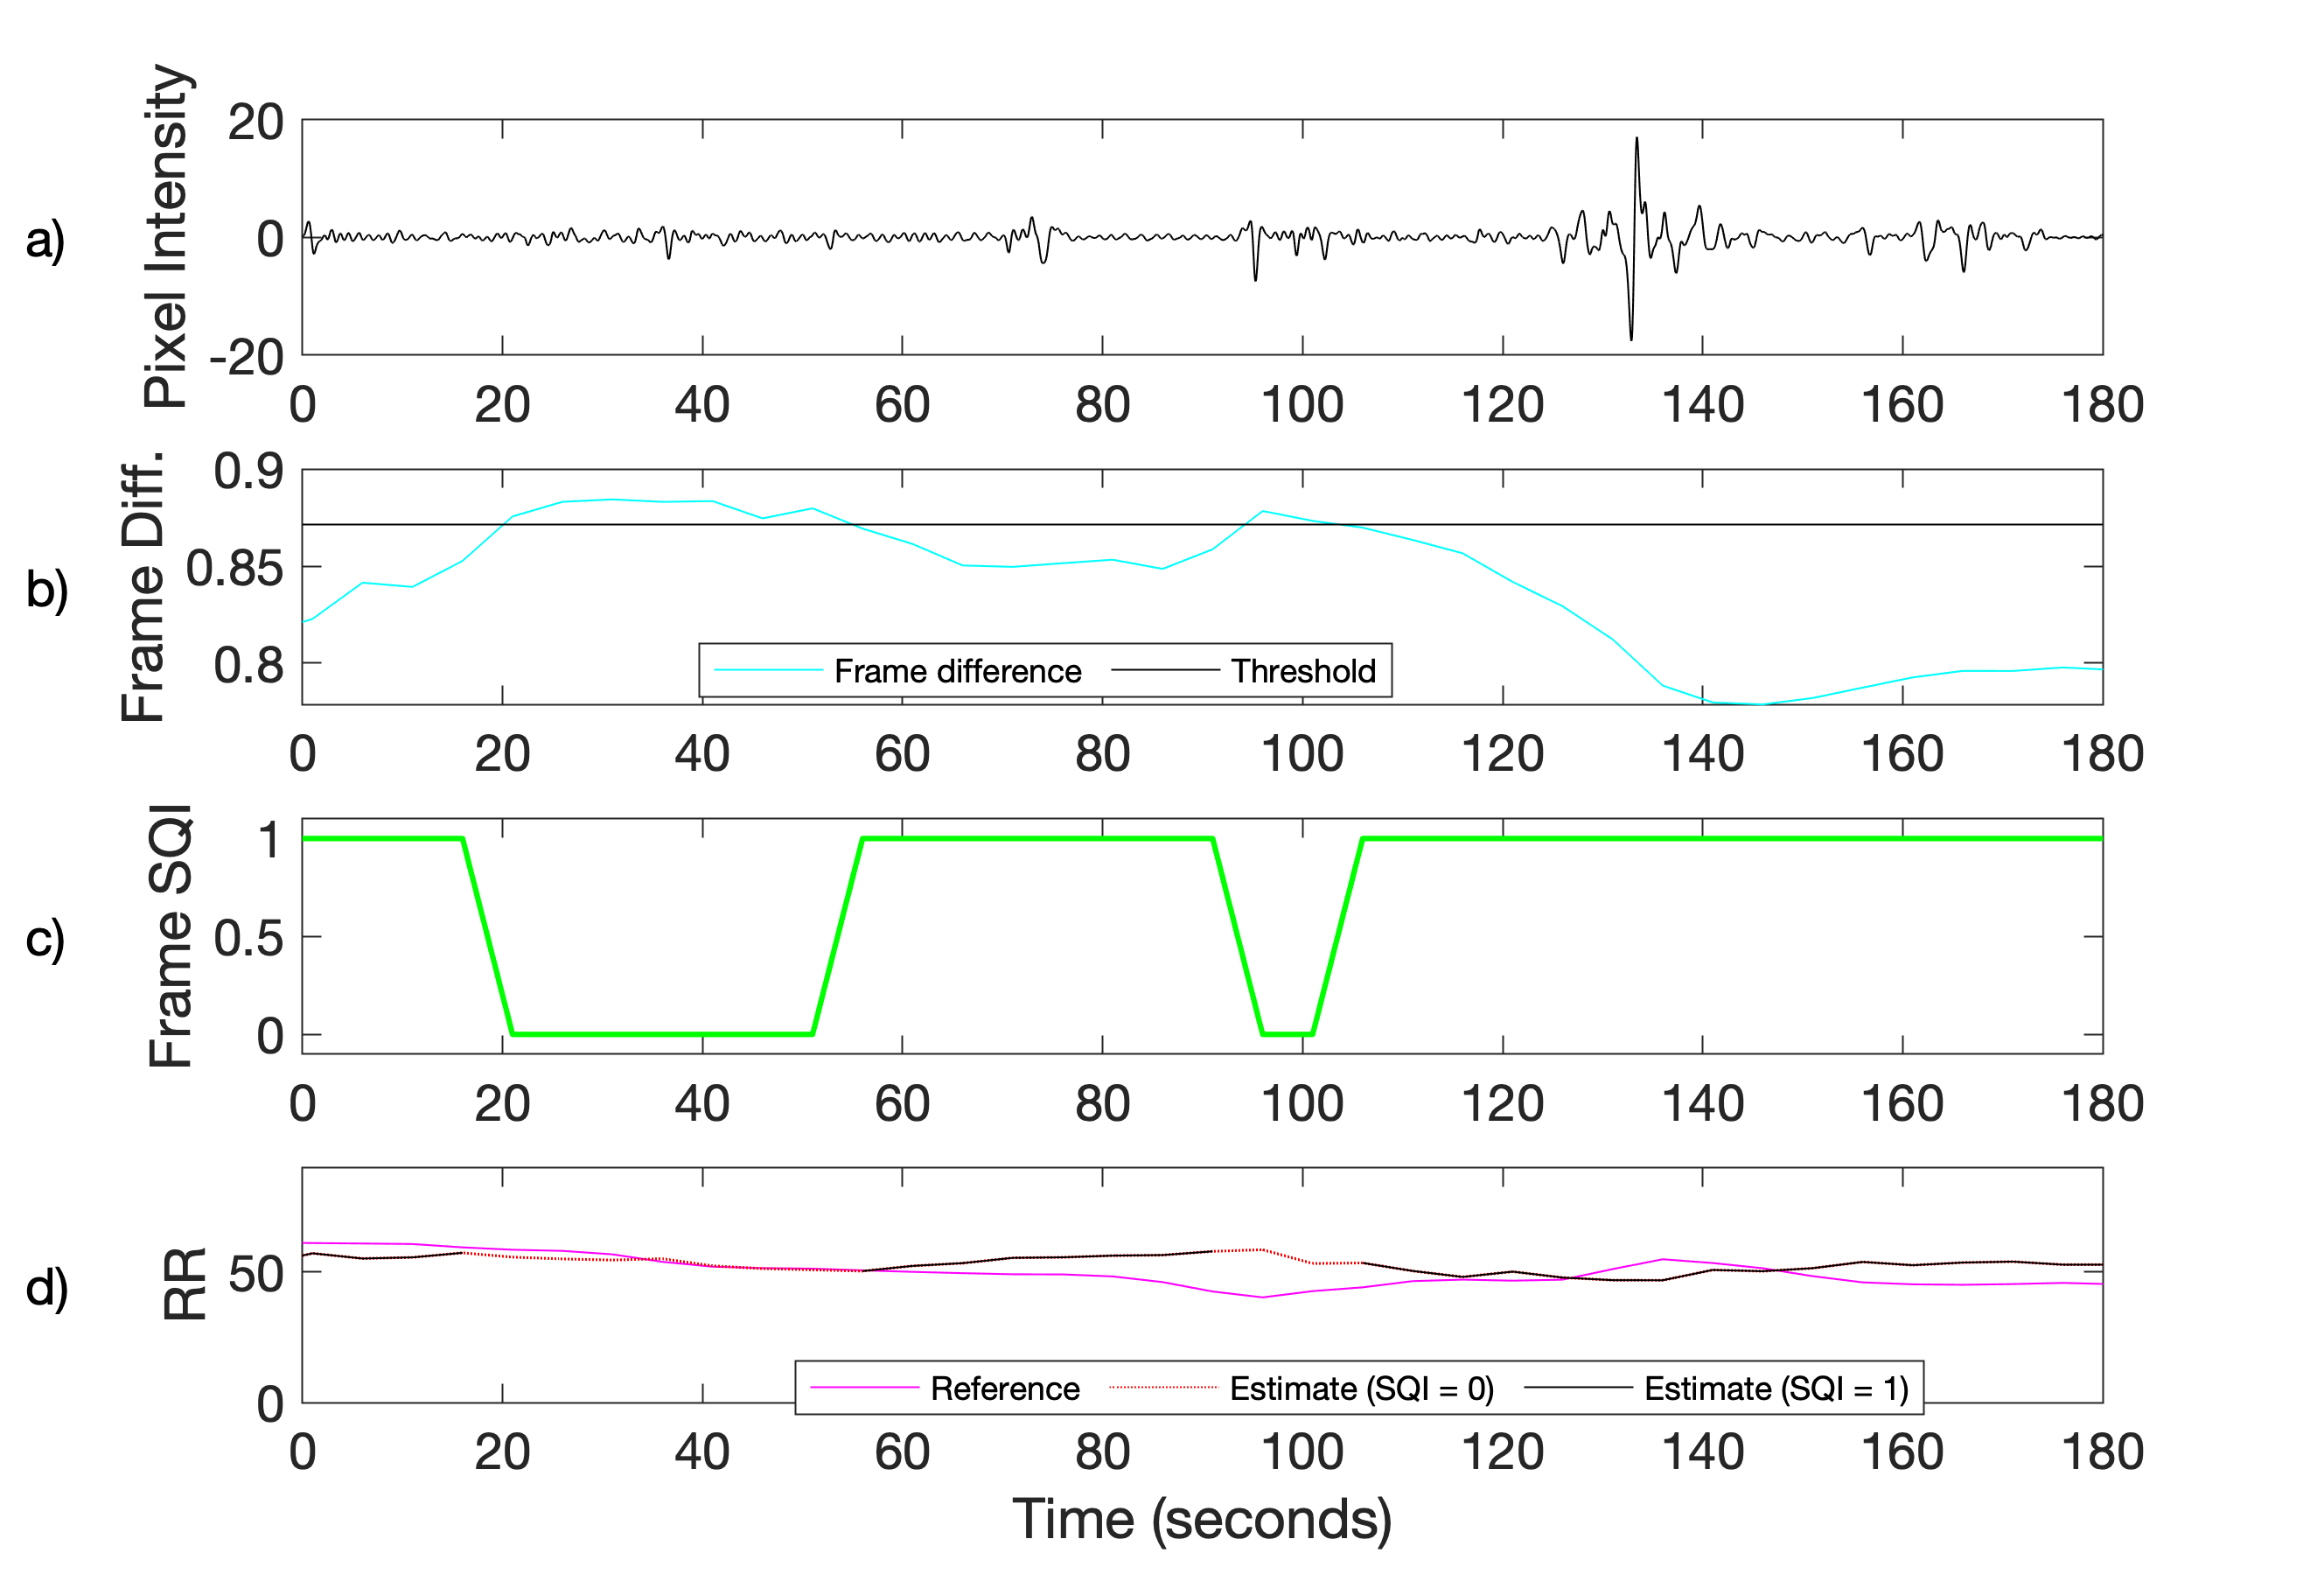
\includegraphics[width=0.6\linewidth,keepaspectratio=true]{nicu_SQI_vidRR.png}
    \caption[Using SQI to discard noisy data. Periods of high movement are removed using signal quality index.]{Using SQI to discard noisy data. Periods of high movement are removed using signal quality index. a) Filtered PPGi signal; b) Frame difference; c) Frame difference SQI; d) Comparison between reference and HR estimate.}
    \label{SQI_vidRR}
\end{figure}

 \subsection{Estimating RR}
 
If the frame difference SQI was set to 1, the peak-to-peak estimate was taken as the final RR estimate for each 40-second window, sliding by 5 seconds. The estimated RR was then compared to the reference values provided by the Philips monitor.

\section{Results}
 \subsection{Heart rate}
 
Figure~\ref{HRresults} shows a comparison between the estimated HR and the reference values reported by the Philips monitor. Figure~\ref{HRsummary} shows a set of summary performance plots for the proposed HR estimation algorithms.
 
\begin{figure}[!ht]
\centering
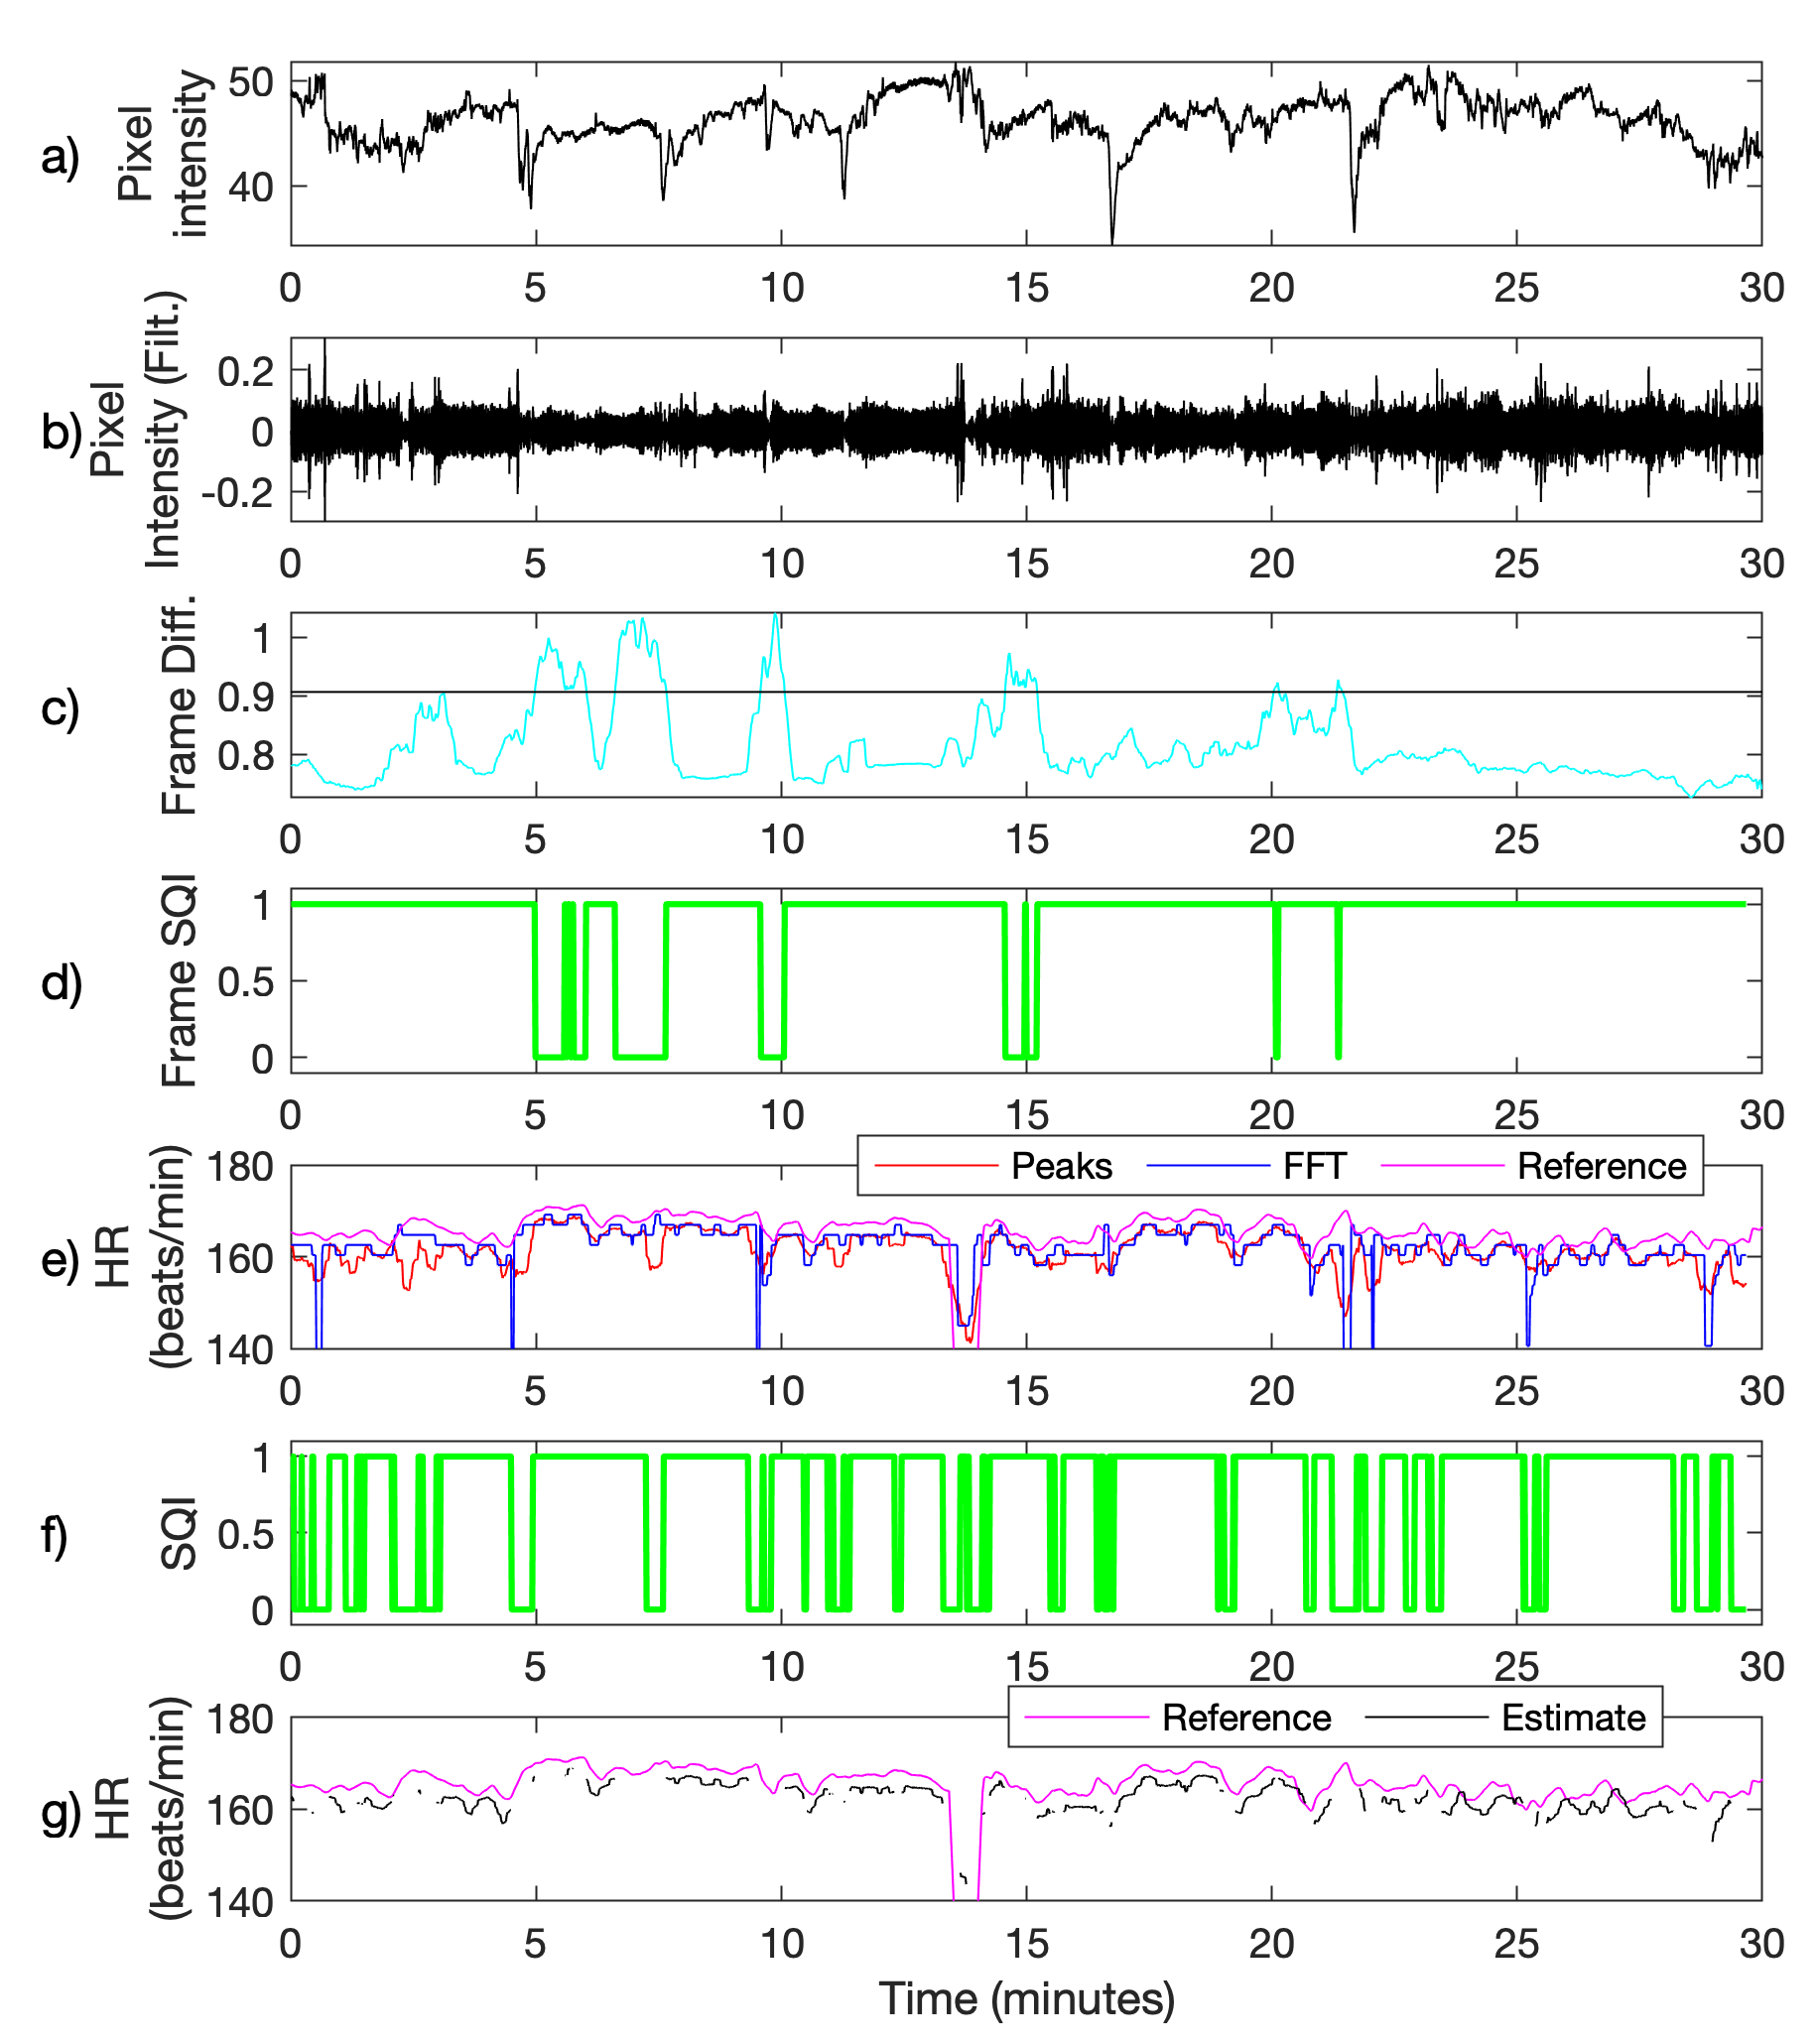
\includegraphics[width=0.6\linewidth,keepaspectratio=true]{nicu_HREstimates.png}
    \caption[Heart rate estimation for a 30-minute recording session.] {Heart rate estimation for a 30-minute recording session. a) Pixel intensity signal; b) Filtered pixel intensity signal; c) Frame difference and d) Frame difference SQI; e) Comparison between reference and peak and FFT estimates; f) Signal difference SQI; g) Comparison between reference and HR estimate.}
     \label{HRresults}
    \end{figure}
 
\begin{figure}[!ht]
    \centering
\includegraphics[width=0.6\linewidth,keepaspectratio=true]{nicu_HR_summary.png}
 \caption[Comparison between the reference and estimated heart rate estimates.]{Comparison between the reference and estimated heart rate estimates. a) Bland-Altman plot; b) Histogram of the differences between the two HR estimates and c) Correlation plot shows a positive correlation between the two measurements. The red line represents the linear fit.}
\label{HRsummary}
\end{figure}
 
 \subsection{Respiratory rate}
 
Figure~\ref{rrestimates} shows a comparison between the estimated RR and the reference values provided by the Philips monitor. Figure~\ref{RRsummary} shows a set of summary performance plots for the proposed RR estimation algorithms.

\begin{figure}[!ht]
\centering
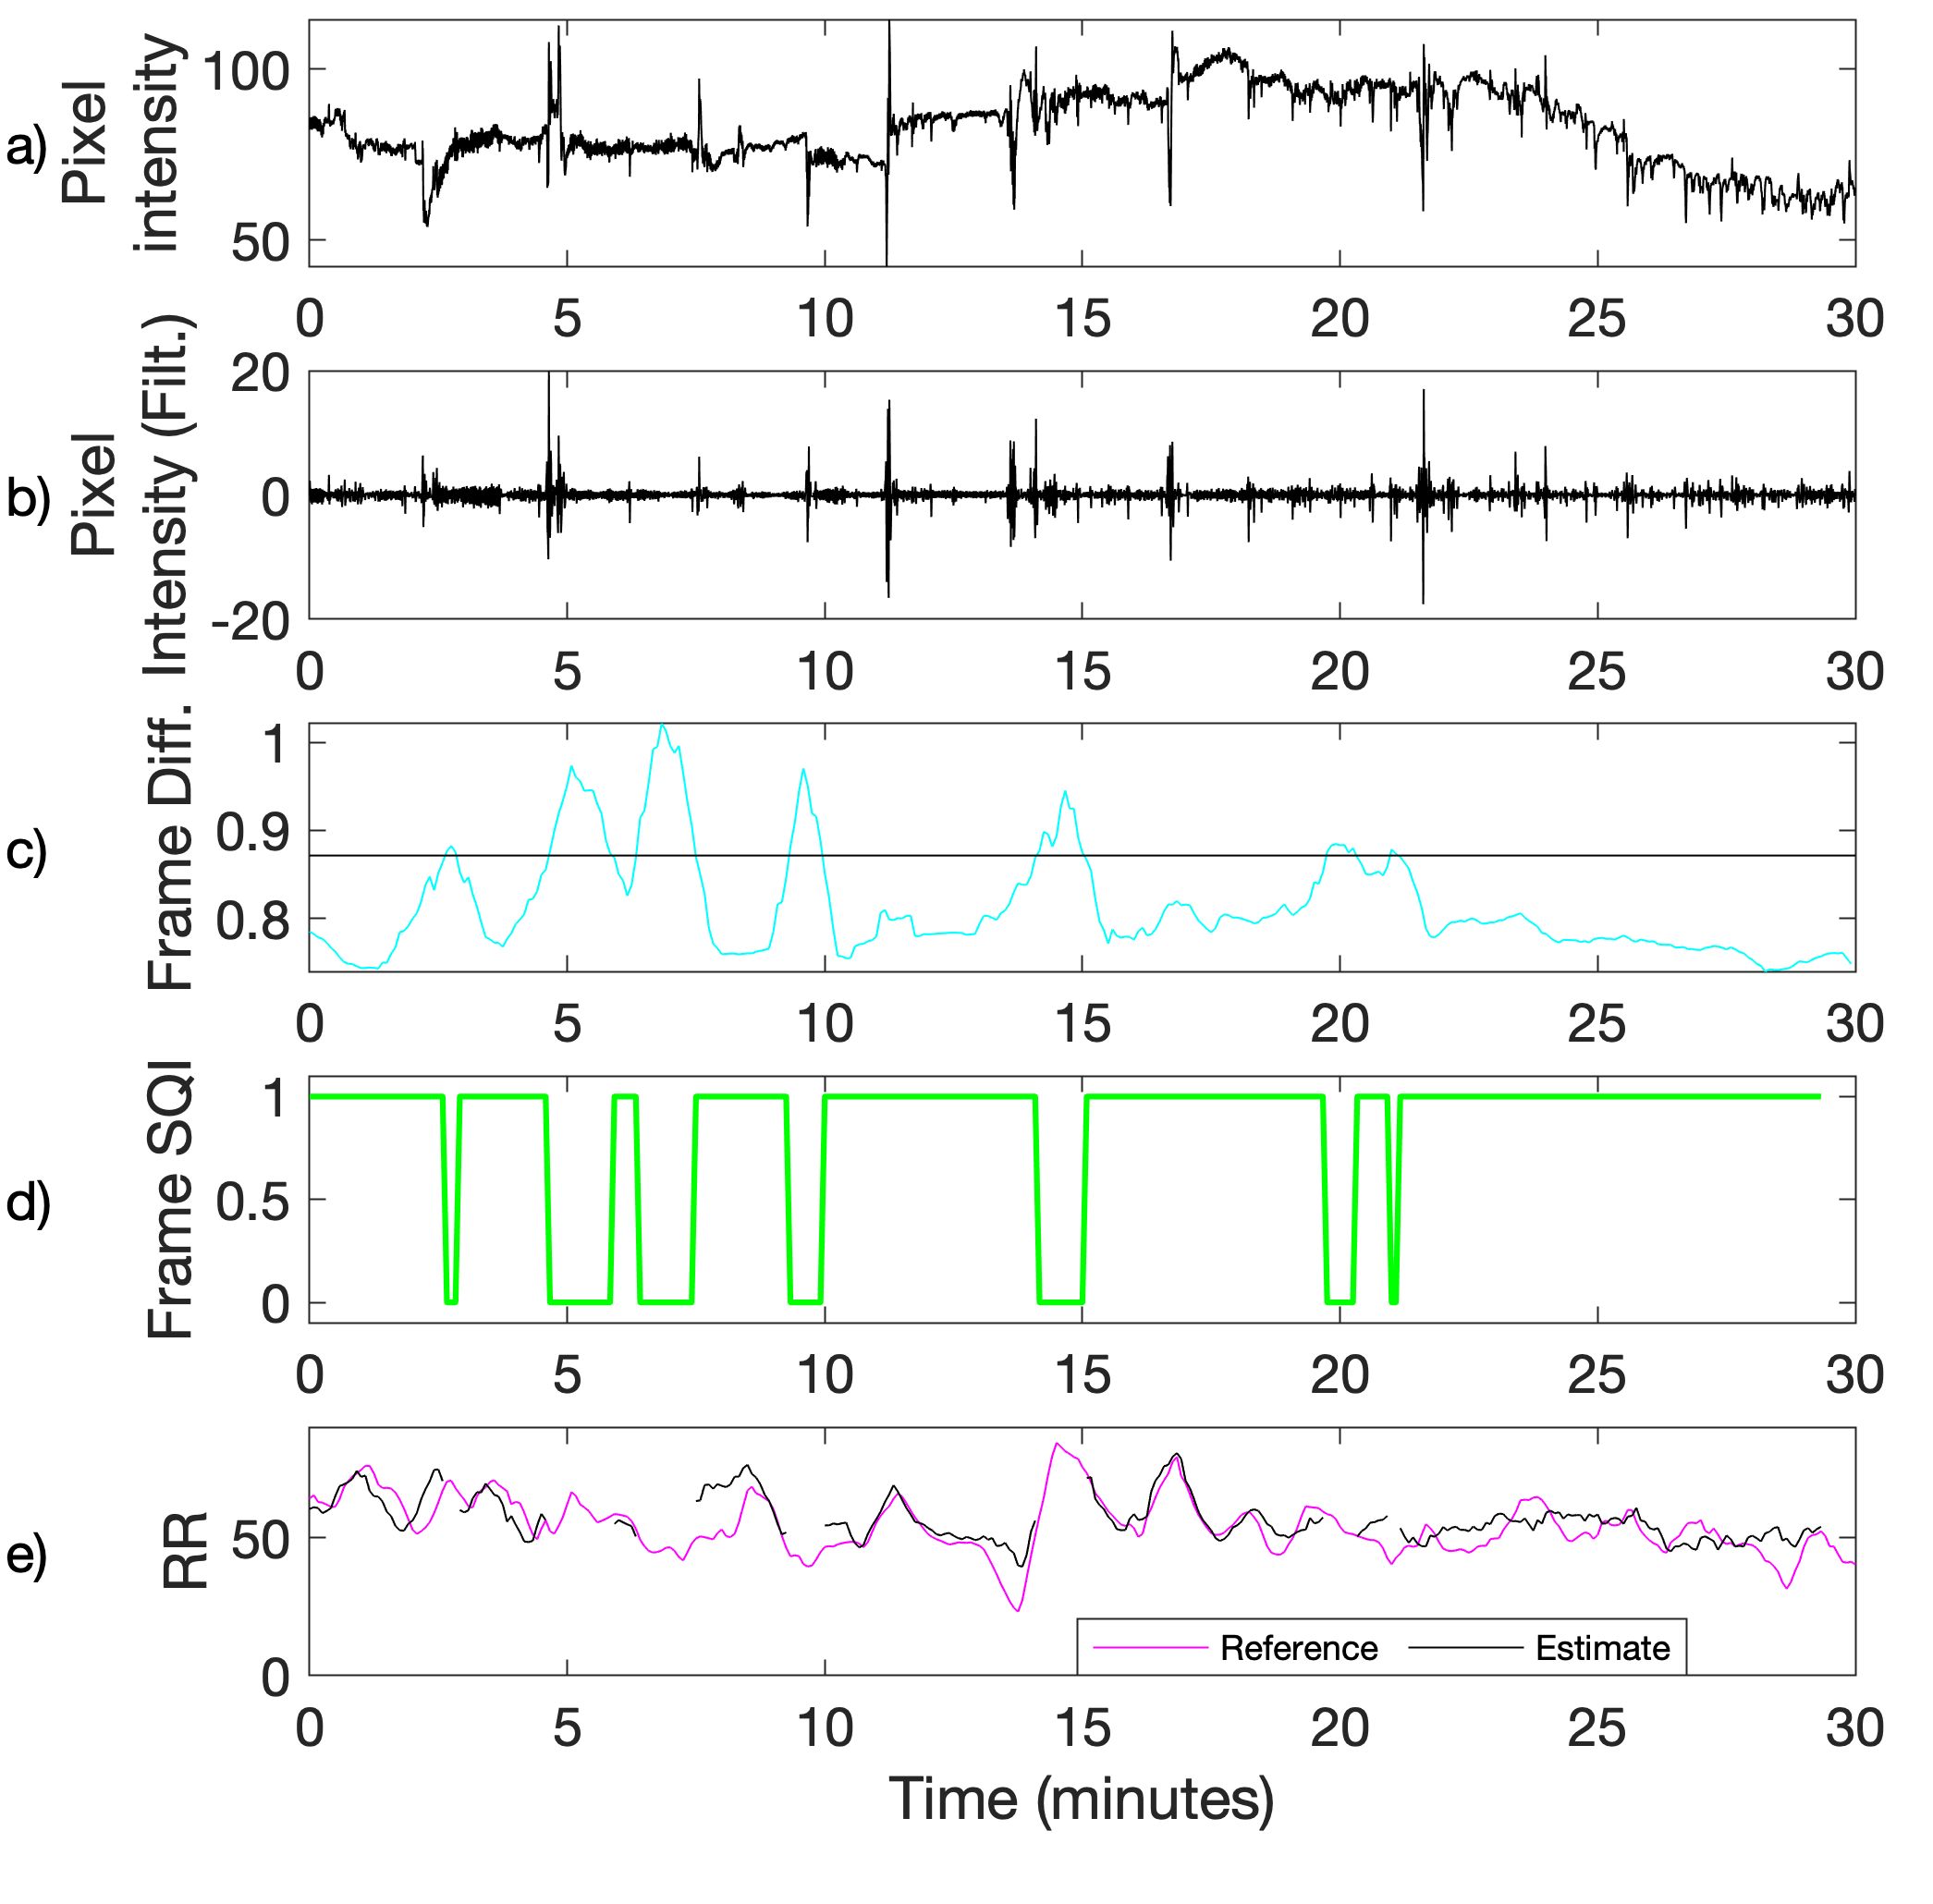
\includegraphics[width=0.6\linewidth,keepaspectratio=true]{nicu_RREstimates.png}
    \caption[Respiratory rate estimation for a 30-minute recording session.]{Respiratory rate estimation for a 30-minute recording session. a) Pixel intensity signal; b) Filtered pixel intensity signal; c) Frame difference and d) Frame difference SQI e) Comparison between reference and RR estimate.}
         \label{rrestimates}
    \end{figure}
 

\begin{figure}[!ht]
    \centering
\includegraphics[width=0.6\linewidth,keepaspectratio=true]{nicu_RR_summary.png}
 \caption[Comparison between the reference and estimated respiratory rate.]{Comparison between the reference and estimated respiratory rate a) Bland-Altman plot. b) Histogram of the differences between the two RR estimates and c) Correlation plot shows a positive correlation between the two measurements. The red line represents the linear fit.}
     \label{RRsummary}
\end{figure}
 
   \subsection{Summary metrics}
   
Table~\ref{RRmetrics} shows overall performance metrics for estimating heart rate and respiratory rate from the video camera for the selected recording session.

 \begin{table}[!ht]
\centering
\caption[Summary of error analysis for the proposed algorithms for RR  and HR computation from video camara data.]{Summary of error analysis for the proposed algorithms for RR and HR computation from video camera data.}
\label{RRmetrics}
\vspace{2em}
\begin{tabular}{p{1.5 cm}|r  r  r  r}
 	 \tableHeaderStart 
	  & MAE* & MAD* & RMSE* & r \\
   	 \midrule
   	   HR &  3.2 & 1.1 &  3.5 & 0.83 \\
       RR &  5.3 & 5.0 & 6.9 & 0.71 \\        
      \bottomrule 
      \tableHeaderEnd
      
       \multicolumn{4}{l}
      {
      \footnotesize * Values in  beats/min for HR or breaths/min for RR
      }\\
\end{tabular}
\end{table}

\section{Discussion}

Heart rate can be estimated from the video camera data because changes in blood volume due to the cardiac cycle lead to subtle color changes in skin recorded by the video camera. As can be seen in figure \ref{HRsummary} and table \ref{RRmetrics}, the estimated heart rate was comparable to the values provided by the reference medical device. The mean bias of 3.2 beats/min and correlation coefficient of 0.83 suggest that our signal processing methods performed adequately. Most of the errors were the result of motion artefacts, caused by the camera moving or clinical interventions by the nurses. The Frame difference SQI was successful in removing most of these periods. The two proposed methods, FFT and beat counting, performed adequately for the whole session selected and, therefore, the SQI did not discard a substantial proportion of the HR estimated data.

To extract a respiratory signal from video camera data, the movement of the nappy and exposed skin was used. Comparisons between RR provided by the Philips monitor and the estimated RR showed varied performance. The correlation coefficient (r = 0.71) and relatively greater errors (MAE of 5.3 and MAD of 5.0) in figure \ref{RRsummary} and table \ref{RRmetrics} respectively, are clear indication of this. Overall, we were able extract and estimate RR using SQIs to isolate time periods with good quality data. It is worth noting when interpreting the results obtained that the estimates provided by the Philips monitor are noisy, clinical staff often compute RR manually.

\section{Conclusion}

In this chapter, video data from a study on premature infants was analysed, employing signal processing methods to extract cardiac and respiratory signals and estimate RR and HR. The study comprised recording video data under a real hospital scenario, regular patient care was not disrupted. The pre-term infants monitored were active and clinical staff routinely interacted with them. This dataset presents a recording scenario that will be comparable to the recordings of children diagnosed with pneumonia in our future clinical study in Kenya. Therefore, the algorithms proposed in this chapter will be expanded and improved during the next phase of my DPhil.

The HR results in this chapter had a positive correlation of 0.83. An RMSE of 3.5 beats/min was achieved using the video camera for HR estimation. RR estimation was also successful, with a correlation coefficient of R= 0.71. An RMSE of 6.9 was achieved from the non-contact RR estimation. The methods developed in this chapter will form the foundation for algorithms to estimate vital signs from video camera data from children diagnosed with pneumonia, which will be developed during the second year of my DPhil.